% \documentclass{article}
% \documentclass[12pt, vietnamese]{report}
\documentclass[12pt, vietnamese]{article}
\usepackage{ngntrgduc}
\usepackage[utf8]{vietnam}
\usepackage[
    a4paper,
    margin=1in,
    footskip=0.75in,
    % top=0.75in,
    % bottom=0.25in,
]{geometry}

\usepackage{bbm} % Indicator function
\usepackage{pgfgantt} % Gantt chart
% \usepackage{titlesec} % Title customization
\usepackage{caption} % Caption alignment
\captionsetup{justification=raggedright,singlelinecheck=false}

\usepackage{multirow}

\usepackage[
    backend=biber,
    % style=alphabetic,
    sorting=none  % Entries are processed in citation order 
    % sorting=ydnt  % sort by year (descending), name, title 
]{biblatex}
\addbibresource{refs.bib}

\hypersetup{
    colorlinks,
    citecolor=magenta,
    linkcolor=black,
    urlcolor=cyan,
    pdftitle={Xử lý dữ liệu khuyết},
    pdfauthor={Trung-Duc Nguyen}
}

\graphicspath{img/}

% \setcounter{chapter}{-1} %Getting chapter numbering to start at 0

 % Header and Footer
% \pagestyle{fancy}
% \fancyhf{}
% \lhead{\leftmark}
% \rhead{\thepage}

\setlength\parindent{0pt}   % new paragraphs will not be indented
% \setlength{\parskip}{0.2cm} % more space between paragraphs
\setlength{\parskip}{0.25cm} % more space between paragraphs

\onehalfspacing % More space each line
% \doublespacing

\newtheorem{thm}{Định lý}[section]
\newtheorem{lemma}{Bổ đề}[section]
% \newtheorem{defi}{Định nghĩa}[chapter]
% \newtheorem{defi}{Định nghĩa}
\newtheorem{defi}{Định nghĩa}[section]
\newtheorem{corollary}{Hệ quả}[section]
% \newtheorem{corollary}{Hệ quả}[section]
% \newtheorem{proof}{Chứng minh}[chapter]
\newtheorem{prop}{Mệnh đề}[section]
\newtheorem{assume}{Giả thiết}[section]
% \newtheorem{prop}{Mệnh đề}
\newtheorem{remark}{Nhận xét}[section]
\newtheorem{example}{Ví dụ}[section]
% \newtheorem{notation}[define]{Kí hiệu}

\numberwithin{equation}{section}
\numberwithin{figure}{section}

  % Define theorems style
\newcommand{\dps}{\displaystyle}
% \newcommand{\E}{\mathrm{E}}
\newcommand{\E}{\mathbb{E}}
\newcommand{\Var}{\mathrm{Var}}
\newcommand{\Cov}{\mathrm{Cov}}
\newcommand{\cov}{\Sigma}
\newcommand{\eps}{\varepsilon}
\newcommand{\Normal}{\mathcal{N}}

\newcommand{\der}{\mathrm{d}}

\newcommand{\NA}{\texttt{NA}}
% \newcommand{\Xobs}[1]{\ensuremath X_{\text{obs}#1}} % Highlight command

% \DeclareMathOperator{\Id}{Id}
% \DeclareMathOperator{\relu}{ReLU}
\newcommand{\relu}{ReLU}
% \operatorname{}

\newcommand{\separator}{\vspace{2ex}\hrule\vspace{2ex}}
  % Symbol shortcuts


\begin{document}

\begin{center}	
    \large{ĐẠI HỌC QUỐC GIA THÀNH PHỐ HỒ CHÍ MINH}\\
    \large{TRƯỜNG ĐẠI HỌC KHOA HỌC TỰ NHIÊN}\\
    \large{KHOA TOÁN - TIN HỌC}
    \vspace{0.5in}
    
    
\includegraphics[scale=0.3]{img/hcmus.png}
    
    \huge{Báo cáo Seminar Phương pháp toán}
    \vspace{0.2in}
    
    {\huge\textbf{Xử lý dữ liệu khuyết}}\\
    \vspace{1in}
\end{center}

\begin{center}
    \begin{tabular}{rl}
        \large Sinh viên thực hiện:& \large\textbf{Nguyễn Trung Đức} \\
        \large Mã số sinh viên:& \large\textbf{21110269} \\
        \large Giảng viên hướng dẫn:& \large\textbf{TS. Hoàng Văn Hà}
    \end{tabular}
\end{center}

\vfill

\begin{center}
    % \large{TP. Hồ Chí Minh - \today}
    \large{TP. Hồ Chí Minh - Ngày 20 tháng 1 năm 2025}
\end{center}

\thispagestyle{empty}
\newpage \ \thispagestyle{empty} \newpage

% Lời cảm ơn
% % \input{acknowledgement}

% Mục lục
\tableofcontents \newpage

% Danh mục các thuật ngữ và từ viết tắt
\section*{Danh mục các thuật ngữ và từ viết tắt}
\addcontentsline{toc}{section}{Danh mục các thuật ngữ và từ viết tắt}

% \subsection*{Thuật ngữ}
\setlength{\tabcolsep}{18pt}
\begin{tabular}{ll}
    \textbf{Thuật ngữ} & \textbf{Ý nghĩa} \\
    \hline
    Bayes predictor & Dự đoán Bayes \\
    Imputation, Impute & Điền khuyết \\
    Features & Đặc trưng \\
    Mask & Che \\
    % Spectral norm & Chuẩn phổ \\
    % Spectral radius & Bán kính phổ \\
    Neural network & Mạng nơ-ron nhân tạo \\
    Activation function & Hàm kích hoạt \\
    Loss function & Hàm mất mát \\
    Learning rate & Tốc độ học \\
    Layer & Lớp (của Neural network) \\
    Hidden layer & Lớp ẩn\\
    Hidden unit & Đơn vị ẩn \\
    Train set & Tập dùng để huấn luyện \\
    Validation set & Tập dùng để đánh giá \\
    Test set & Tập dùng để kiểm tra \\
    Epoch & Một lần duyệt qua hết các dữ liệu trong train set \\
    Batch size & Số lượng mẫu dữ liệu trong một lần huấn luyện \\
\end{tabular}

% \subsection*{Từ viết tắt}

\setlength{\tabcolsep}{18pt}
\begin{tabular}{ll}
    \textbf{Từ viết tắt} & \textbf{Ý nghĩa} \\
    \hline
    MCAR & Missing Completely At Random \\
    MAR & Missing At Random \\
    MNAR & Missing Not At Random \\
    EM & Expectation Maximization \\
    LR & Linear Regression \\
    MLP & Multilayer perceptron \\
    KNN & K-Nearest Neighbors \\
    SVM & Support vector machine \\
    PCA & Principal Component Analysis \\
    MICE & Multiple Imputation by Chained Equations \\
    GAN & Generative adversarial network \\
    % VAE & Variational Autoencoder \\
    MSE & Mean Squared Error \\
\end{tabular}



\newpage

% \listoftables 
% \listoffigures

% Tóm tắt
\section*{Tóm tắt}
% \addcontentsline{toc}{section}{\protect\numberline{}Tóm tắt}
\addcontentsline{toc}{section}{Tóm tắt}

Bài báo \cite{le2020neumiss} xử lý vấn đề dữ liệu khuyết trong các bài toán học có giám sát, cụ thể là các bài toán hồi quy tuyến tính.
Dựa trên việc xấp xỉ dự đoán Bayes (mô hình dự đoán tốt nhất theo lý thuyết) trên tập dữ liệu khuyết,
bài báo đề xuất sử dụng chuỗi Neumann kết hợp với phương pháp Algorithm Unrolling \cite{gregor2010unroll} để xây dựng một kiến trúc neural network có tên là NeuMiss. Mạng NeuMiss sử dụng các hàm kích hoạt phi tuyến là các mask (chỉ số) của dữ liệu khuyết, giúp mạng hoạt động hiệu quả với các tập dữ liệu có độ lớn trung bình trở lên với các cơ chế dữ liệu khuyết khác nhau 
bao gồm cơ chế dữ liệu khuyết hoàn toàn ngẫu nhiên (MCAR), cơ chế dữ liệu khuyết ngẫu nhiên (MAR), và cơ chế dữ liệu khuyết không ngẫu nhiên (MNAR).
Đặc biệt, mạng NeuMiss hoạt động hiệu quả trong những trường hợp mà các phương pháp truyền thống thường gặp khó khăn.

Mục đích của bài báo cáo này là đi trình bày lại các kiến thức nền tảng và kiến trúc của mạng NeuMiss, cũng như một số kết quả thực nghiệm cho các cài đặt khác nhau.


% Kiến thức chuẩn bị
\section{Kiến thức chuẩn bị}

Trong mục này, chúng tôi trình bày một số kiến thức chuẩn bị cho các nội dung được nghiên cứu trong các phần sau.

\begin{comment}
    \section{Hàm Gauss}
    Hàm Gauss là một hàm số có dạng cơ sở là:
    \[
        f(x) = \exp \left( -x^2 \right), 
    \]
    
    và có dạng tham số là:
    \[
        f(x) = a \exp \left(- \dfrac{1}{2} \dfrac{(x-b)^2}{c^2}\right),
    \]
    
    với tham số $a$ là độ cao, $b$ là vị trí của đỉnh, và $c$ điều khiển độ rộng của đồ thị hàm số.
    
    Trong xác suất thống kê, hàm Gauss thường được dùng để biểu diễn cho hàm mật độ xác suất của phân phối chuẩn:
    \[
        f(x) = \dfrac{1}{\sigma \sqrt{2\pi}} \exp \left( -\dfrac{1}{2} \dfrac{(x-\mu)^2}{\sigma^2} \right),
    \]
    với $\mu$ là trung bình và $\sigma^2$ là phương sai của phân phối.
    
    % Ngoài ra, ta còn có thể viết dưới dạng
    % \[
    %     f(x) = \dfrac{1}{\sigma \sqrt{2\pi}} \exp \left( -\dfrac{1}{2} \dfrac{(x-\mu)^2}{\sigma^2} \right),
    % \]    
\end{comment}



\subsection{Phân phối chuẩn đa biến}
Phân phối chuẩn đa biến $X \sim \Normal(\mu, \cov)$ với vector trung bình là $\mu \in \R^d$ và ma trận hiệp phương sai đối xứng, nửa xác định dương $\cov \in \R^{d \times d}$, có 
% pdf 
hàm mật độ xác suất
như sau:
\[
    f(x | \mu, \cov) 
    % \Normal(x | \mu,\cov)
    % f_X(x)
    = \frac{1}{\sqrt{(2\pi)^{d} |\cov|}}  \exp \left(- \frac{1}{2} (x - \mu)^{T} \cov^{-1}  (x - \mu)\right), \ x \in \R^d,
\]
với $|\cov|$ là định thức của $\cov$.

% \begin{draft}
\textbf{Lý do sử dụng phân phối chuẩn đa biến cho bài toán xử lý dữ liệu khuyết?}

\begin{itemize}
    \item Nhiều phương pháp thống kê dựa trên giả định dữ liệu có phân phối chuẩn, dễ làm việc hơn vì được nghiên cứu lâu dài, cùng với Định lý giới hạn trung tâm khiến cho phân phối chuẩn được sử dụng rộng rãi.
    \item Dữ liệu thực tế thường có nhiều cột đặc trưng (features), dẫn đến dữ liệu có số chiều cao, nên ta cần một phân phối có khả năng xử lý dữ liệu nhiều chiều và cho ta thấy được mối tương quan giữa các đặc trưng với nhau.
    \item Phân phối chuẩn đa biến cho phép mô hình hoá các phân phối xác suất đồng thời của các đặc trưng khác nhau.
    % (?)
\end{itemize}
% \end{draft}

Trong khuôn khổ bài báo cáo này, từ giờ về sau, hàm mật độ xác suất của phân phối chuẩn đa biến sẽ được gọi là hàm Gauss để cho thuận tiện.

\begin{lemma}\label{lem:prod_gauss} (Tích của hai hàm Gauss là một hàm Gauss)

    Cho $f(x) = \exp\left(-\dfrac{1}{2}(x - a)^{\top} A^{-1} (x - a)\right)$ 
    và $g(x) = \exp\left( -\dfrac{1}{2} (x - b)^{\top} B^{-1} (x - b)\right)$ là hai hàm Gauss, với $A$ và $B$ là ma trận nửa xác định dương, ta có:
    \[
        f(x)g(x)=\exp\left(-\frac{1}{2}(a-b)^{\top}(A+B)^{-1}(a-b)\right)
        \exp\left(-\frac{1}{2}(x-\mu_{p})^{\top}\cov_{p}^{-1}(x-\mu_{p})\right),
    \]
    với $\mu_p$ và $\cov_p$ 
    lần lượt là vector trung bình và ma trận hiệp phương sai của tích hai hàm Gauss, 
    phụ thuộc vào $a$, $A$, $b$, và $B$.
\end{lemma}

\begin{proof}
    % Phần chứng minh của bổ đề này có thể tìm thấy ở trong 
    Xem mục A.2 trong bài báo \cite{le2020neumiss}.
\end{proof}

\begin{comment}
\begin{proof}
    Với $f(X)$ có phân phối chuẩn đa biến $\Normal(X | a, A)$, ta có:
    \begin{align*}
        f(X) &= \exp\left(-\dfrac{1}{2}(X - a)^{\top} A^{-1} (X - a)\right) \\
        % &= \exp((X - a)^{\top} (A^{-1}X - A^{-1}a )) \\
        &= \exp\left(-\dfrac{1}{2}(X^{\top}A^{-1}X - X^{\top}A^{-1}a - a^{\top} A^{-1}X + a^{\top}A^{-1}a) \right)\\
        &= \exp\left( -\dfrac{1}{2}(X^{\top}A^{-1}X - 2X^{\top}A^{-1}a + a^{\top}A^{-1}a) \right).
    \end{align*}
    Qua đây, ta thấy được $A^{-1}$ là nghịch đảo của phương sai, $A^{-1}a$ là tích của nghịch đảo phương sai với trung bình của $X$, và $a^{\top}A^{-1}a$ là hằng số. Tiếp theo ta sẽ thấy được sự tương đồng đối với trường hợp $f(X)g(X)$.
    
    Ta xét:
    \begin{align}
        f(X)g(X) &= \exp\left(-\dfrac{1}{2}(X - a)^{\top} A^{-1} (X - a)\right) \exp\left(-\dfrac{1}{2}(X - b)^{\top} B^{-1} (X - b)\right) \notag \\
        &= \exp\left(-\dfrac{1}{2}\left((X - a)^{\top} A^{-1} (X - a) + (X - b)^{\top} B^{-1} (X - b)\right) \right) \notag \\
        &= \exp\left(-\dfrac{1}{2}\left( X^{\top}A^{-1}X - 2X^{\top}A^{-1}a + a^{\top}A^{-1}a + 
        X^{\top}B^{-1}X - 2X^{\top}B^{-1}b + b^{\top}B^{-1}b\right) \right) \notag \\
        &= \exp\left( -\dfrac{1}{2} \left(X^{\top}(A^{-1} + B^{-1})X - 2X^{\top}(A^{-1}a + B^{-1}b) + a^{\top}A^{-1}a + b^{\top}B^{-1}b \right) \right). \label{eq:fxgx}
    \end{align}
    Với $\mu_p$ và $\cov_p$ 
    lần lượt là vector trung bình và ma trận hiệp phương sai của tích hai hàm Gauss, ta đặt:
    \begin{align*}
        \cov_{p}^{-1} &= A^{-1} + B^{-1}, \\
        \cov_{p}^{-1} \mu_p &= A^{-1}a + B^{-1}b.
    \end{align*}
    Thay vào \eqref{eq:fxgx}, ta có:
    \begin{align*}
        f(X)g(X) &= \exp \left( -\dfrac{1}{2} \left(X^{\top}\cov_p^{-1}X - 2X^{\top}\cov_p^{-1} \mu_p + a^{\top}A^{-1}a + b^{\top}B^{-1}b\right) \right) \\
        &= \exp \left( -\dfrac{1}{2} \left(X^{\top}\cov_p^{-1}X - 2X^{\top}\cov_p^{-1} \mu_p + \mu_{p}^{\top} \cov_p^{-1}\mu_p - \mu_{p}^{\top} \cov_p^{-1}\mu_p  + a^{\top}A^{-1}a + b^{\top}B^{-1}b\right) \right) \\
        &= \exp\left( -\dfrac{1}{2} \left(X^{\top}\cov_p^{-1}X - 2X^{\top}\cov_p^{-1} \mu_p + \mu_{p}^{\top} \cov_p^{-1}\mu_p \right) \right) \\
         &\quad \quad \times \exp\left( -\dfrac{1}{2} \left(a^{\top}A^{-1}a + b^{\top}B^{-1}b - \mu_{p}^{\top} \cov_p^{-1}\mu_p \right) \right)\\
        &= \exp\left( -\dfrac{1}{2}\left(a^{\top}A^{-1}a + b^{\top}B^{-1}b - \mu_{p}^{\top} \cov_p^{-1}\mu_p \right) \right) \exp\left( -\dfrac{1}{2} (X-\mu_p)^{\top}\cov_p^{-1}(X - \mu_p)\right).
    \end{align*}
    Giờ ta đi đơn giản phần hệ số ở phía trước:
    \begin{align}
        c &= a^{\top}A^{-1}a + b^{\top}B^{-1}b - \mu_{p}^{\top} \cov_p^{-1}\mu_p \notag \\
        &= a^{\top}A^{-1}a + b^{\top}B^{-1}b - 
        \left(a^{\top}A^{-1}(A^{-1}+B^{-1})^{-1}+b^{\top}B^{-1}(A^{-1}+B^{-1})^{-1}\right) (A^{-1}a + B^{-1}b) \notag \\
        &= a^{\top}(A^{-1}-A^{-1}(A^{-1} + B^{-1})^{-1}A^{-1})a+b^{\top}(B^{-1}-B^{-1}(A^{-1}+B^{-1})^{-1}B^{-1})b \notag \\
        &\quad \quad -2a^{\top} (A^{-1} (A^{-1} + B^{-1})^{-1} B^{-1} )b.
        % \quad \quad \quad \text{(Do } A \text{ và } B \text{ đối xứng)} 
        \label{eq:need_woodbury}
    \end{align}
    Ta có Woodbury Identity (Đồng nhất thức Woodbury) cho các ma trận có thể nhân hoặc cộng được với nhau (conformable) $A, B, C, D$ dưới dạng:
    \[
        \displaystyle \left(A+CBD\right)^{-1} = A^{-1}-A^{-1}C\left(B^{-1}+DA^{-1}C\right)^{-1}DA^{-1}.
    \]
    Việc khai triển phương trình trên có thể tìm thấy ở \cite{ridgway2006matrixwoodbury}. Khi $C = D = I$, ta được:
    \[
        \left(A+B\right)^{-1}=A^{-1}-A^{-1}\left(B^{-1}+A^{-1}\right)^{-1}A^{-1}.
    \]
    Thay vào \eqref{eq:need_woodbury}, ta được
    \begin{align*}
        c &= a^{\top} (A+B)^{-1} a + b^{\top}(A + B)^{-1}b 
        -2a^{\top} (A^{-1} (A^{-1} + B^{-1})^{-1} B^{-1} )b \\
        &= a^{\top} (A+B)^{-1} a + b^{\top}(A + B)^{-1}b -2a^{\top} \left(B(A^{-1} + B^{-1})A \right)^{-1}b \\
        &= a^{\top} (A+B)^{-1} a + b^{\top}(A + B)^{-1}b -2a^{\top} \left(BA^{-1}A + BB^{-1}A \right)^{-1}b \\
        &= a^{\top} (A+B)^{-1} a + b^{\top}(A + B)^{-1}b -2a^{\top} \left(B + A \right)^{-1}b \\
        &= (a-b)^{\top} (A+B)^{-1} (a-b).
    \end{align*}
    Vậy 
    \[
        f(X)g(X) = \exp\left(-\dfrac{1}{2}(a-b)^{\top} (A+B)^{-1} (a-b)\right) 
        \exp\left(-\dfrac{1}{2}(X-\mu_p)^{\top}\cov_p^{-1}(X - \mu_p)\right) \qed
    \]
\end{proof}
\end{comment}


\subsection{Phân phối chuẩn có điều kiện}
Một tính chất quan trọng của phân phối chuẩn đa biến đó là nếu $2$ tập hợp biến ngẫu nhiên có phân phối chuẩn đa biến đồng thời (Joint Gaussian), thì phân phối có điều kiện của một tập khi biết tập còn lại cũng là một phân phối chuẩn đa biến, tức 
\[
    f(x_a | x_b) = \Normal(x_a | \mu_{a|b}, \cov_{a|b}).
\]

Giả sử $x$ là vector $d$ chiều có phân phối chuẩn đa biến $\Normal(x|\mu, \cov)$. Ta chia $x$ thành $2$ tập con riêng biệt $x_a$ và $x_b$ được cho bởi \[
x = \begin{pmatrix}
    x_a \\
    x_b
\end{pmatrix}.
\]
Lúc này $x$ cũng được gọi là phân phối chuẩn đa biến bị chia  (Partitioned Multivariate Gaussian).
Ta cũng định nghĩa vector trung bình 
\[
\mu = \begin{pmatrix}
    \mu_a \\
    \mu_b
\end{pmatrix},
\]
và ma trận hiệp phương sai 
\[
\cov = \begin{pmatrix}
    \cov_{aa} & \cov_{ab} \\
    \cov_{ba} & \cov_{bb} \\
\end{pmatrix}.
\]

Ta có: 
\[
    \begin{split}
        \mu_{a|b} &= \mu_a + \cov_{ab}\cov_{bb}^{-1} (x_b - \mu_b), \\ 
        \cov_{a|b} &= \cov_{aa} - \cov_{ab} \cov_{bb}^{-1} \cov_{ba}.
    \end{split}
\]

\begin{proof}
    Xem mục 2.3.1 của \cite{bishop2006pattern} hoặc \cite{statexconditionalgaussian}. \qed
\end{proof}

Ngoài ra, nếu ma trận hiệp phương sai $\cov_{ab} = 0$, ta có $\mu_{a|b} = \mu_a$, $\cov_{a|b} = \cov_{aa}$, tức $x_a$ và $x_b$ độc lập với nhau, với $P(x_a|x_b) = P(x_a)$. Tức là khi ta lấy tích của các biến ngẫu nhiên độc lập với nhau, ta chỉ cần lấy các phần tử đường chéo của ma trận hiệp phương sai $\cov$.


\subsection{Chuẩn ma trận (Induced vector norm)}
Với chuẩn $2$ của vector $x = (x_1, \dots, x_n) \in \R^n$ có dạng:
\[
    \|x\|_2 = \sqrt{ \sum_{i=1}^n x_{i}^2}
    = \sqrt{x^{\top} x}
    = \sqrt{\langle x, x \rangle},
\] ta xét chuẩn 2 (induced-2 norm) cho ma trận $A$, hay còn được biết đến là chuẩn phổ (spectral norm):
\[
    \|A\|_2 = \max_{x \neq 0} {\frac{\|Ax\|_2}{\|x\|_2}}
    = \max_{\substack{x \neq 0 \\ \|x\|_2 = 1}} {\|Ax\|_2} = 
    \sigma_{max} (A),
\]

với $\sigma_{max} (A)$ là giá trị suy biến (singular value) lớn nhất của $A$. Và khi $A$ đối xứng, xác định dương, thì giá trị suy biến tương ứng với lại trị riêng của ma trận, tức $\|A\|_2 = \lambda_{\max}$.


\subsection{Chuỗi Neumann}
Chuỗi Neumann thường làm việc với các toán tử trong các không gian hàm. Nhưng trong khuôn khổ bài báo cáo, ta chỉ cần làm việc với ma trận -- toán tử biến đổi tuyến tính.

Với ma trận $A \in \R^{d \times d}$, chuỗi Neumann của $A$ được biểu diễn dưới dạng
\begin{equation*}
    \sum_{k=0}^{\infty} A^k = I + A + A^2 + \dots,
\end{equation*}
với $I$ là ma trận đơn vị.
Chuỗi Neumann hội tụ với điều kiện chuẩn phổ 
của ma trận $A$ bé hơn $1$ ($\|A\|_2 < 1$).
Và khi chuỗi hội tụ, tồn tại nghịch đảo của $(I - A)$ với:
\begin{equation*}
    (I - A)^{-1} = \sum_{k=0}^{\infty} A^k.
\end{equation*}

Để chứng minh điều trên, ta xét:
\[
    S_n = \sum_{k=0}^n A^k.
\]

Ta có:
\[
    \lim_{n \to \infty }(I - A) S_{n}
    =\lim_{n \to \infty} \left(\sum_{k=0}^{n}A^{k} - \sum_{k=0}^{n}A^{k+1}\right)
    =\lim_{n \to \infty} \left(I-A^{n+1}\right) = I.
\]
Vậy nghịch đảo của $I-A$ là chuỗi Neumann của $A$.

Từ đây, chuỗi Neumann có thể được sử dụng để xấp xỉ nghịch đảo của một ma trận: Xét ma trận $A$ khả nghịch, ta có:
\begin{equation*}
    \begin{split}
        A^{-1} &= (I - I + A)^{-1}\\
        &= (I - (I - A))^{-1}\\
        &= (I - T)^{-1}, \\
    \end{split}
\end{equation*}
với $T = I - A$. Nếu $T$ thoả điều kiện $\|T\|_2 < 1$, thì ta có theo chuỗi Neumann:
\[
    (I - T)^{-1} = \sum_{k=0}^{\infty} T^k.  
\]
Và do đó:
\begin{equation*}
    A^{-1} = (I - (I - A))^{-1} = \sum_{k=0}^{\infty} (I - A)^k.
\end{equation*}

Vì với điều kiện $\|I-A\|_2 < 1$, $I-A$ dần hội tụ khi $k \to \infty$, nên chuỗi chặt cụt (truncated) tại $l$ hữu hạn có thể cho ta 1 xấp xỉ nghịch đảo ma trận tốt.
\begin{equation*}
     A^{-1} \approx \sum_{k=0}^{l}(I-A)^{k}.
\end{equation*}



\subsection{Bán kính phổ}
Cho ma trận $A \in \C^{d \times d}$ với các trị riêng $\lambda_1, \dots, \lambda_d$, bán kính phổ (spectral radius) $\rho (A)$ của $A$ là giá trị tuyệt đối trị riêng lớn nhất của ma trận $A$:
\[
    \rho (A) = \max\{|\lambda_1|, \dots, |\lambda_d|\}.
\]

Khi $A$ là ma trận thực đối xứng, bán kính phổ của $A$ bằng với chuẩn phổ của $A$:
\[
    \rho (A) = \|A\|_2 = \lambda_{\max}.
\]

\subsection{Tỷ số Rayleigh (Rayleigh quotient)}
Tỷ số Rayleigh thường được sử dụng để xấp xỉ trị riêng của ma trận thực đối xứng $A$ dưới dạng: 
\[
    r(x) = \dfrac{x^{\top} A x}{x^{\top} x},
\]
với $x \neq 0$.

Để cho đơn giản, ta cho $\|x\| = 1$, lúc này, việc tìm trị riêng lớn nhất của $A$ có dạng:
\[
    \lambda_{\max}(A) = \rho(A) =  \max_{\substack{\|x\|=1}} x^{\top} A x.
\]


Người đọc có thể đọc thêm về phần kiến thức này ở phần \MakeUppercase{\romannumeral 5} trong \cite{trefethennumerical}.


% \section{Law of total expectation (Luật kỳ vọng đầy đủ)}
% Law of total expectation (hay Law of iterated expectation) cho ta biết rằng kỳ vọng của một biến ngẫu nhiên bằng với lại tổng các kỳ vọng của biến ngẫu nhiên đó dựa trên một biến ngẫu nhiên khác. 

% Với biến ngẫu nhiên $X$, $Y$, ta có
% \[
%     \E\left[\E[X|Y]\right] = \E [X].
% \]



\subsection{Phép nhân Hadamard (Hadamard product)}
Trong các phép toán ma trận, phép nhân Hadamard, ký hiệu là $\odot$, là phép nhân từng phần tử (element-wise) của 2 ma trận với nhau. 

Xét $A \in \R^{m \times n}$ và $B \in \R^{m \times n}$, với lần lượt $a_{ij}$, $b_{ij}$ nằm ở dòng thứ $i$ và cột thứ $j$ của ma trận $A$, $B$. Phép nhân Hadamard của ma trận $A$ và $B$ là:
\[
    \mathbf{A} \odot \mathbf{B} =
    \begin{bmatrix}
        a_{11}  b_{11} & a_{12}  b_{12} & \dots  & a_{1n}  b_{1n} \\
        a_{21}  b_{21} & a_{22}  b_{22} & \dots  & a_{2n}  b_{2n} \\
        \vdots & \vdots & \ddots & \vdots \\
        a_{m1}  b_{m1} & a_{m2}  b_{m2} & \dots  & a_{mn}  b_{mn}
    \end{bmatrix}.
\]


\subsection{Điểm bất động}
Điểm bất động (fixed point) $x^*$ là điểm thoả 
\[
    f(x^*) = x^*,
\]
với hàm $f$ cố định. Nói cách khác, điểm bất động là điểm không thay đổi với 1 phép biến đổi cho trước.


\subsection{Algorithm Unrolling}
Ý tưởng của Algorithm Unrolling được giới thiệu lần đầu trong công trình của Gregor và LeCun \cite{gregor2010unroll}, nhằm liên kết các thuật toán lặp (Iterative algorithms) với các neural networks. Cụ thể, mỗi vòng lặp trong thuật toán được mô hình hóa như một lớp (layer) trong mạng, qua đó thuật toán lặp được biểu diễn như một chuỗi các lớp liên tiếp. Việc truyền qua mạng tương đương với việc thực thi thuật toán lặp một số lần hữu hạn.

\begin{figure}[h]
    \centering
    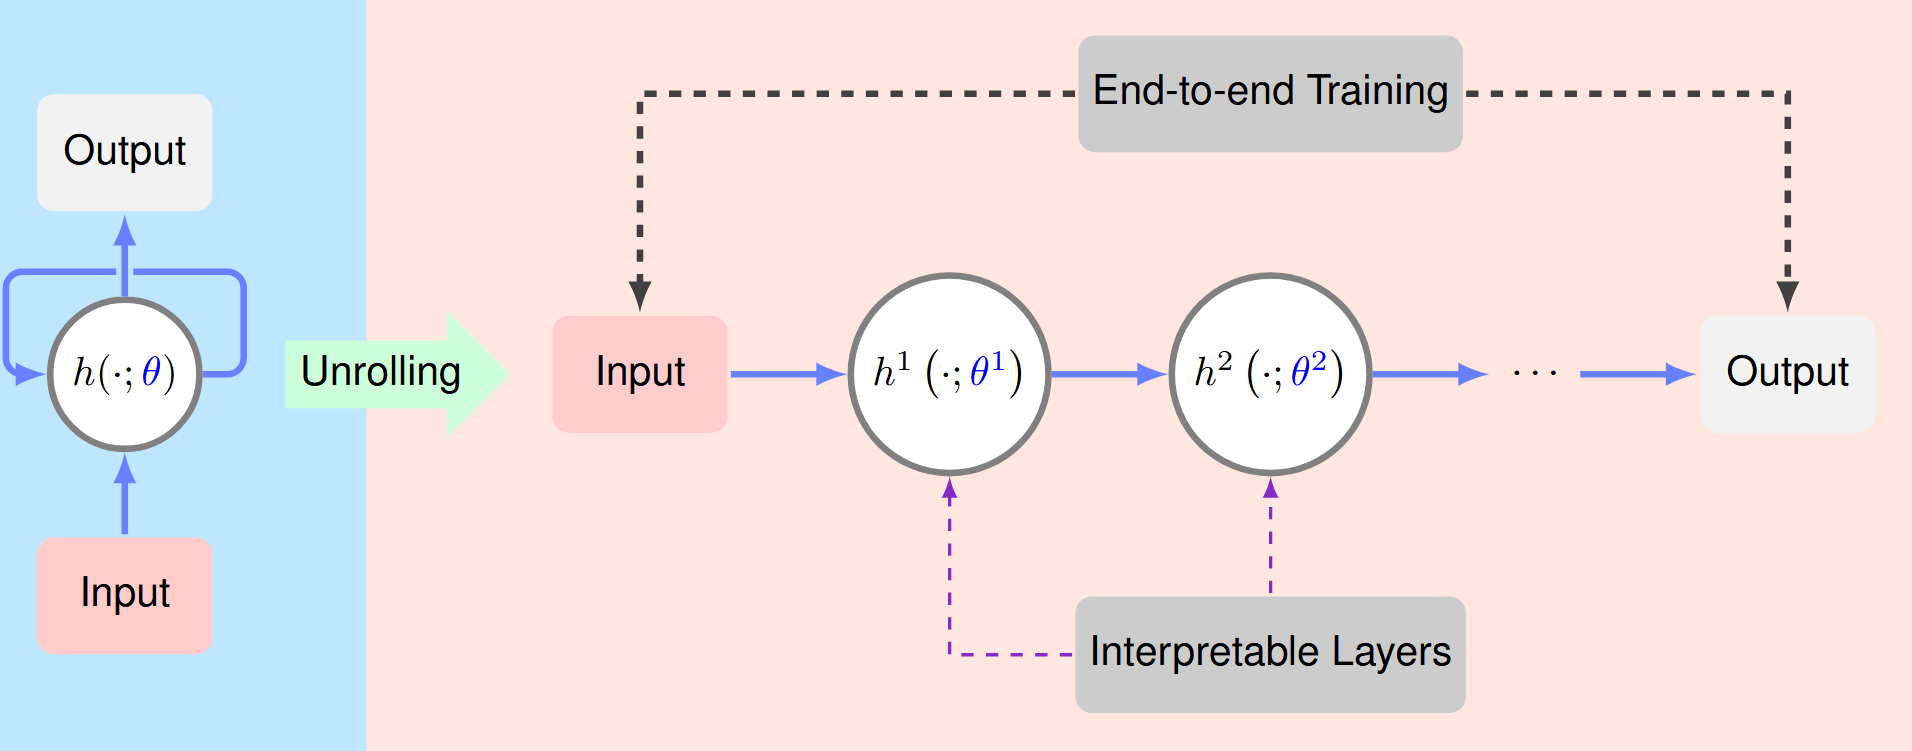
\includegraphics[width=\textwidth]{img/unrolling.png}
    \caption{
        \textbf{Tổng quan Algorithm unrolling:} cho một thuật toán lặp (bên trái), một neural network tương ứng (bên phải) có thể được tạo bằng cách ``trải'' các phép lặp $h$ ra. 
        Phép lặp $h$ 
        % (bên trái) 
        được thực thi với số lần hữu hạn, tương ứng với các lớp $h^1, h^2, \dots$ của mạng. Mỗi phép lặp $h$ phụ thuộc vào tham số $\theta$, và tham số này được 
        % truyền vào 
        biểu diễn bởi tham số của
        mạng dưới dạng $\theta^1, \theta^2, \dots$. Thay vì phải xác định các tham số một cách thủ công trong thuật toán lặp, ta học $\theta^1, \theta^2, \dots$ trực tiếp từ quá trình huấn luyện mô hình. Bằng cách này, mạng có thể đạt được hiệu suất tốt hơn so với thuật toán lặp ban đầu. Ngoài ra, các lớp của mạng được kế thừa tính diễn giải (interpretability) một cách tự nhiên từ quá trình lặp.
        Các tham số có thể học được có màu xanh.
        (được trích dẫn từ~\cite{monga2021unroll})
    }
    \label{fig:unrolling}
\end{figure}


% Nội dung
\section{Giới thiệu về xử lý dữ liệu khuyết}
Dữ liệu bị khuyết là một vấn đề phổ biến trong lĩnh vực Khoa học dữ liệu, đặc biệt với các bài toán học có giám sát (supervised learning). Mục tiêu chính của các bài toán này là dự đoán các giá trị hoặc phân loại các dữ liệu mới dựa trên các đặc trưng từ dữ liệu cũ. Phần lớn các phương pháp nhằm giải quyết các bài toán này đều được thiết kế để hoạt động trên tập dữ liệu hoàn chỉnh. Do đó, khi dữ liệu đầu vào bị khuyết, mô hình không thể học đầy đủ các quy luật cần thiết để có thể hoạt động tốt, làm giảm chất lượng của mô hình. Vậy nên ta cần tiền xử lý các giá trị bị khuyết, hoặc sử dụng các mô hình có thể tự xử lý dữ liệu khuyết 
trên các tập dữ liệu không hoàn chỉnh.

% xử lý dữ liệu khuyết khá giống với bài toán học bán giám sát khi mà dữ liệu được học không đầy đủ, nhưng các bài toán dữ liệu khuyết khác semi-supervised learning ở chỗ label của dữ liệu có thể bị khuyết, trong khi trong semi-supervised learning thì không


\subsection{Các cơ chế dữ liệu khuyết} \label{section:missingmechanism}
Dữ liệu bị khuyết có thể đến từ nhiều nguyên nhân khác nhau, ví dụ như: do người trả lời không cung cấp thông tin, do quá trình khảo sát không thu thập đủ dữ liệu, do lỗi ở phía thiết bị hoặc phần mềm thu thập dữ liệu, do quá trình xử lý dữ liệu,... Do đó, các dữ liệu khuyết cũng nên được chia ra theo từng loại dựa trên nguyên nhân gây ra dữ liệu bị khuyết để có cách xử lý phù hợp. Việc sử dụng những phương pháp xử lý không phù hợp với từng loại dữ liệu khuyết có thể dẫn tới kết luận sai lệch từ dữ liệu.

Theo Donald B. Rubin, dữ liệu khuyết được chia thành 3 loại chính: MCAR, MAR, và MNAR \cite{rubin1976inference}.

\begin{itemize}
    \item \textbf{Dữ liệu khuyết hoàn toàn ngẫu nhiên (Missing Completely At Random -- MCAR)} là dữ liệu bị khuyết hoàn toàn không phụ thuộc vào dữ liệu quan sát được hoặc không quan sát được. Hay nói cách khác, việc dữ liệu bị khuyết là ``hoàn toàn ngẫu nhiên''.

% Ví dụ: Một máy cảm biến thu nhập dữ liệu bỗng dưng bị hỏng không rõ nguyên nhân, làm cảm biến không thể hoạt động và thu thập dữ liệu, thì dữ liệu ở trong khoảng thời gian đó bị khuyết theo cơ chế MCAR. -> chưa chắc
    
    Ví dụ: Trong một khảo sát nghiên cứu, một số phiếu trả lời bị thất lạc ngẫu nhiên do quá trình vận chuyển của bưu điện. Việc thất lạc phiếu khảo sát là hoàn toàn ngẫu nhiên và không liên quan đến nội dung câu trả lời, người tham gia, hoặc bất kỳ yếu tố nào khác trong khảo sát.

% Đây là dạng dữ liệu khuyết dễ xử lý nhất, bởi vì nó không tạo ra bất cứ bias nào cho việc phân tích và suy diễn dữ liệu. 

    \item \textbf{Dữ liệu khuyết ngẫu nhiên (Missing At Random -- MAR)} là dữ liệu bị khuyết chỉ phụ thuộc vào dữ liệu quan sát được mà không phụ thuộc vào dữ liệu không quan sát được (hay chính nó).

    Ví dụ: Trong một khảo sát có các câu hỏi về chủ đề nhạy cảm, phụ nữ thường ngại và không trả lời các câu hỏi nhạy cảm, có thể là do họ không thoải mái với câu hỏi đó. Tuy nhiên, đàn ông thì không có xu hướng như vậy và sẵn lòng trả lời. Như vậy, dữ liệu bị khuyết theo cơ chế MAR vì việc thiếu dữ liệu về câu trả lời của các câu hỏi nhạy cảm phụ thuộc vào giới tính của người được khảo sát, chứ không phải do giá trị của chính các câu hỏi nhạy cảm.


    \item \textbf{Dữ liệu khuyết không ngẫu nhiên (Missing Not At Random -- MNAR)} là dữ liệu bị khuyết không thuộc một trong hai cơ chế dữ liệu khuyết bên trên, tức dữ liệu bị khuyết phụ thuộc vào dữ liệu quan sát được và không quan sát được, hoặc chỉ phụ thuộc vào dữ liệu dữ liệu không quan sát được, hay chính nó.

    MNAR thường xảy ra do người cung cấp thông tin từ chối tiết lộ thông tin cá nhân hay thông tin nhạy cảm.

% Ví dụ: Trong lúc đại dịch COVID-19, địa phương sẽ khảo sát những nhà nào đang có người mắc COVID. Thì một số trường hợp sẽ không điền câu trả lời vào khảo sát (do sợ bị cách ly, xa gia đình,...) có thể sẽ cung cấp nhiều thông tin hữu ích. Lúc này, dữ liệu sẽ bị khuyết theo cơ chế MNAR.

    Ví dụ: Trong một cuộc khảo sát về sức khỏe tâm lý, người tham gia được yêu cầu trả lời câu hỏi về mức độ trầm cảm của họ. Tuy nhiên, những người có mức độ trầm cảm cao thường có xu hướng không trả lời hoặc từ chối cung cấp thông tin về tình trạng của mình do cảm giác lo ngại, xấu hổ, hoặc sợ bị đánh giá. Tức dữ liệu bị khuyết phụ thuộc trực tiếp vào chính giá trị của mức độ trầm cảm.

% Ví dụ: Trong một cuộc khảo sát về mức thu nhập của các hộ gia đình, các hộ gia đình có thu nhập cao thường từ chối trả lời câu hỏi về thu nhập. Điều này có nghĩa là dữ liệu bị thiếu về thu nhập không phải là ngẫu nhiên mà có liên quan trực tiếp đến giá trị thực tế của biến bị thiếu (tức là, những người có thu nhập cao có xu hướng không tiết lộ thu nhập của mình).
\end{itemize}

Với MNAR, ta cần phải mô hình cơ chế dữ liệu khuyết vì sự khuyết dữ liệu có thể cung cấp nhiều thông tin hữu ích.
MNAR thường phức tạp hơn MCAR hay MAR bởi dữ liệu bị khuyết phụ thuộc vào chính nó, không phải do ngẫu nhiên. Chính vì vậy, cơ chế MNAR thường xuất hiện ở trong thực tế, nhưng do nó khó xử lý nên phần lớn các phương pháp xử lý dữ liệu khuyết đều giả định dữ liệu bị khuyết với cơ chế MCAR và MAR, và các phương pháp này thường không thể áp dụng cho MNAR.


\subsection{Phương pháp xử lý dữ liệu khuyết}
Xử lý dữ liệu khuyết là một vấn đề đã được nghiên cứu trong khoảng thời gian dài. Các nhà nghiên cứu đã đề xuất nhiều phương pháp khác nhau, và thường sẽ có 3 hướng xử lý dữ liệu khuyết chính:
\begin{itemize}
    \item Loại bỏ toàn bộ các dữ liệu bị khuyết (Listwise deletion).
    \item Điền khuyết (Impute) dữ liệu bằng các phương pháp điền khuyết.
    \item Sử dụng các phương pháp có thể tự xử lý dữ liệu khuyết hay không bị ảnh hưởng bởi dữ liệu khuyết.
\end{itemize}


Thông thường, cách đơn giản để xử lý dữ liệu khuyết là xoá tất cả các dòng có chứa những dữ liệu khuyết để tập dữ liệu khuyết trở thành tập dữ liệu đầy đủ. 
Nhưng việc xoá tất cả dữ liệu khuyết sẽ khiến tập dữ liệu nhỏ đi, từ đó dữ liệu sẽ không còn nhiều thông tin hữu ích, chưa kể có một số loại dữ liệu khuyết phụ thuộc vào dữ liệu đã quan sát được, hay dữ liệu bị khuyết không hoàn toàn ngẫu nhiên, sẽ cung cấp nhiều thông tin hữu ích như mục \ref{section:missingmechanism} có đề cập.

Từ đó, việc xoá tất cả dữ liệu khuyết không phải là phương pháp tốt trong nhiều trường hợp vì nó có thể bỏ qua những dữ liệu có ích. Thay vào đó, ta sẽ muốn chèn dữ liệu vào những chỗ mà dữ liệu bị khuyết, hay còn được gọi là phương pháp điền khuyết (Imputation).

Điền khuyết
là phương pháp điền dữ liệu khuyết bằng các giá trị cố định. Có nhiều cách để điền khuyết dữ liệu như: Simple Impute (Điền khuyết đơn giản), Interactive Impute (Điền khuyết tuần tự), Multiple Impute (Đa điền khuyết), MICE (Multiple Imputation by Chained Equations), PCA (Principal Component Analysis), hay sử dụng các thuật toán Machine learning như: Random Forest, KNN, Decision Tree, SVM,... không cần giả định về phân phối của dữ liệu do chúng đều là các phương pháp phi tham số.

Tuy nhiên, điền khuyết trong một số trường hợp cũng không phải lựa chọn tốt, khi mà nó có thể thay đổi phân phối của dữ liệu, làm mất tính liên kết giữa các đặc trưng với nhau.

Cùng với sự phát triển của các neural network, một số công trình nghiên cứu đã tận dụng sức mạnh của các kiến trúc mạng khác nhau để xử lý các vấn đề với dữ liệu khuyết,...
ví dụ như: 
MLP (Multilayer perceptron), 
GAIN hay MisGAN (sử dụng kiến trúc GAN để điền khuyết dữ liệu), 
MIWAE (dựa trên Variational Autoencoder),... 

Nhưng những phương pháp này cần có nhiều dữ liệu đầu vào hơn so với các phương pháp điền khuyết trên, cũng như các cơ chế dữ liệu khác nhau thường đòi hỏi các cách xử lý khác nhau.

Trong thực tế, các nhà phân tích dữ liệu thường phải giả sử 1 trong 3 loại cơ chế dữ liệu khuyết vì họ không biết rằng dữ liệu bị khuyết thực tế sẽ thuộc vào kiểu cơ chế nào. Bài báo \cite{le2020neumiss} đề xuất một neural network có thể xử lý đồng thời cả 3 loại cơ chế trong bài toán hồi quy tuyến tính, mà không cần các bước điền khuyết truyền thống.

% \section{Mô hình với dữ liệu khuyết}
\section{Tổng quan các mô hình nghiên cứu với dữ liệu khuyết}
Để mô hình hoá vấn đề dữ liệu khuyết trong các bài toán hồi quy tuyến tính, ta định nghĩa một số ký hiệu:

Ta xét tập dữ liệu $D_n = \{(X_1, Y_1),\dots, (X_n, Y_n)\}$ gồm các cặp $(X_i, Y_i)$ độc lập với nhau, được phân phối theo cặp tổng quát $(X, Y)$, trong đó $X \in \R^d$ đại diện cho vector đặc trưng với $d$ chiều, gồm các biến độc lập, và biến phụ thuộc $Y \in \R$.

Ta định nghĩa vector chỉ mục (indicator vector) $M \in \{0, 1\}^d$, sao cho với mọi $1 \leq j \leq d$:
\[
    M_j = 
    \begin{cases}
        1, \ \text{nếu } X_j \text{ bị khuyết}, \\
        0, \ \text{nếu } X_j \text{ không bị khuyết}. \\
    \end{cases}
\]

Lúc này, vector ngẫu nhiên $M$ đóng vai trò như một mask cho các giá trị dữ liệu bị khuyết trên $X$.

Ta kí hiệu $\mathcal{X} \in \R^d$ là không gian đầu vào,
$\widetilde{\mathcal{X}}$ là không gian tương tự như $\mathcal{X} = (\R \cup \{\NA\})^d$ nhưng có chứa thêm phần tử $\NA$ tượng trưng cho dữ liệu bị khuyết.

Ta kí hiệu vector đặc trưng bị khuyết $\widetilde{X} \in \widetilde{\mathcal{X}}$, sao cho với mọi $1 \leq j \leq d$:
\[
    \widetilde{X}_j = 
    \begin{cases}
    \NA, \text{ nếu } M_j = 1, \\
    X_j, \text{ nếu } M_j = 0. \\
    \end{cases}
\]

Với giá trị hiện thực (realization), ký hiệu là chữ cái in thường: $m$ của $M$, ta ký hiệu:
\begin{align*}
    obs(m) &\text{ là các chỉ số của các giá trị } 0 \text{ của } m \text{ (các giá trị không bị khuyết)}, \\
    mis(m) &\text{ là các chỉ số của các giá trị khác } 0 \text{ của } m \text{ (các giá trị bị khuyết)}.
\end{align*}

Trong ngữ cảnh dữ liệu bị khuyết:
\begin{align*}
    X_{obs(M)} &\text{ là các giá trị quan sát được trong } X, \\
    X_{mis(M)} &\text{ là các giá trị không quan sát được trong } X.
\end{align*}


\begin{example}
Giả sử với giá trị hiện thực: $x = (1.1, 2.2, -3.5, 4, 5.6) \in X$, ta có:
\[
    \begin{split}
        \widetilde{x} &= (1.1, \texttt{NA}, -3.5, 4, \texttt{NA}) \\
        m &= (0, 1, 0, 0, 1) \\
        obs(m) &= (0, 2, 3) \\
        x_{obs(m)} &= (1.1, -3.5, 4) \\
        mis(m) &= (1, 4) \\
        x_{mis(m)} &= (2.2, 5.6). \\
    \end{split}
\]
\end{example}
Khi không có sự nhầm lẫn nào, ta bỏ phần phụ thuộc $m$ để tiện ký hiệu, 
ví dụ như $X_{obs}$ thay vì $X_{obs(m)}$.

\subsection{Hồi quy tuyến tính với dữ liệu khuyết}
Ta xét mô hình hồi quy tuyến tính tổng quát với các biến độc lập $X_1, X_2, \dots, X_d \in \R$, biến phụ thuộc $Y \in \R$, hệ số hồi quy $\beta_0, \beta_1, \dots, \beta_d$, và sai số ngẫu nhiên $\eps \sim \Normal(0, \sigma^2)$:
\begin{equation*}
    Y = \beta_0 + \beta_1 X_1  + \beta_2 X_2 + \dots + \beta_d X_d + \eps,
\end{equation*}

hay ta có thể viết dưới dạng 
\begin{equation*}
    Y = \beta_0 +  \sum_{j=1}^d \beta_j X_j + \eps = \beta_0 + \langle X, \beta \rangle + \eps,
\end{equation*}

với 
$\beta = (\beta_1, \beta_2, \dots, \beta_d) \in \R^d$, $X = (X_1, X_2, \dots, X_d) \in \R^d$, và $\langle \cdot, \cdot \rangle$ là tích vô hướng.


Giả sử quá trình sinh dữ liệu của $Y$ được xác định bởi mô hình hồi quy tuyến tính cho dữ liệu đầy đủ $X$ như sau:
\begin{equation}\label{eq:lr_matrix_notation}
    Y 
    % = f^*(X) + \eps
    = \beta_0^* + \langle X, \beta^* \rangle + \eps,
\end{equation}
với $\beta_0^*$, $\beta^* = (\beta_1^*, \beta_2^*, \dots, \beta_d^*)$ là các hệ số chính xác (true coefficients) để xây dựng mô hình.

% Tuy nhiên, 
Do dữ liệu $X$ có thể bị khuyết, nên việc ước lượng các hệ số hồi quy của mô hình có thể trở nên khó khăn. Đặc biệt khi với số chiều $d$ lớn, hay với các mẫu (pattern) dữ liệu khuyết phức tạp theo $m$.
Thay vào đó, ta sẽ tìm một hàm $f$ mà nó ánh xạ dữ liệu 
bị khuyết $\widetilde{X}$ 
thành giá trị $Y$, tức $f$ là mô hình đưa ra dự đoán dựa trên dữ liệu 
bị khuyết~$\widetilde{X}$.


Vậy làm sao để biết $f$ sẽ cho ra kết quả dự đoán tốt nhất? Kết quả dự đoán tốt nhất khi sai số của dữ liệu được dự đoán $f(\widetilde{X})$ và dữ liệu quan sát $Y$ là nhỏ nhất. Ở đây, ta sử dụng hàm mất mát (loss function) bình phương sai số (squared error) có dạng:
\[
    L (Y, f(\widetilde{X})) = (Y - f(\widetilde{X}))^2.
\]

Tiếp theo, ta muốn $f$ hoạt động tốt trên toàn bộ tập dữ liệu $D_n$, bao gồm cả tập test, chứ không phải chỉ riêng 1 điểm dữ liệu. Do hàm mất mát chỉ dùng để đo sai số của 1 giá trị dự đoán, nên ta lấy kỳ vọng (trung bình) của hàm mất mát để giảm sai số dự đoán trung bình trên các điểm dữ liệu để đánh giá độ tốt của mô hình:
\[
    \E [L(Y, f(\widetilde{X}))] = \E[(Y - f(\widetilde{X}))^2],
\]
% hay còn được biết đến là Mean Squared Error (MSE).
Kỳ vọng của hàm mất mát ngoài ra còn có một tên gọi khác là hàm rủi ro (risk).
Vì ta muốn mô hình $f$ đưa ra dự đoán tốt nhất dựa trên dữ liệu khuyết $\tilde{X}$,
tức mô hình có hàm rủi ro đạt giá trị thấp nhất (còn được gọi là Bayes risk),
nên ta đi giải quyết bài toán tối ưu:
\begin{equation}\label{eq:bayes_predictor_optimization_form}
    f_{\widetilde{X}}^* \in \argmin_{f: \widetilde{\mathcal{X}} \to \R} \E [(Y - f(\widetilde{X}))^2].
\end{equation}

Phương trình này nhắm tới việc tìm $f_{\tilde{X}}^*$ sao cho khi áp dụng vào dữ liệu bị khuyết $\tilde{X}$, nó sẽ đưa ra dự đoán trung bình gần nhất có thể với giá trị thực của $Y$. 
Lúc này, $f_{\widetilde{X}}^*$ còn được gọi là dự đoán Bayes (Bayes predictor).
Hay có thể nói, dự đoán Bayes $f_{\widetilde{X}}^*$ là mô hình dự đoán $Y$ tốt nhất dựa trên dữ liệu khuyết $\widetilde{X}$.

% Sở dĩ lại có ``Bayes'' trong Bayes risk và dự đoán Bayes là do chúng được dùng để tính toán cái chưa biết trên phân phối của dữ liệu đã được biết trước.

Do $\widetilde{\mathcal{X}}$ tồn tại những phần tử $\NA$ đại diện cho dữ liệu khuyết, nên ta khó có thể tính toán~$f$ dựa trên $\widetilde{X}$. Từ đây, ta
viết lại phương trình của dự đoán Bayes \eqref{eq:bayes_predictor_optimization_form}
dưới dạng kỳ vọng có điều kiện của giá trị $Y$ với dữ liệu bị khuyết $\widetilde{X}$ để dễ tính toán:
\begin{align}
    f_{\widetilde{X}}^* (\widetilde{X})
    &= \E [Y | \widetilde{X}] \notag \\
    &= \E \left[Y | M,X_{obs(M)}\right] \notag \\
    &= \sum_{m \in \{0,1\}^{d}} \E\left[Y|X_{obs(m)}, M=m\right] \mathbbm{1}_{M=m}. \label{eq:bayes_predictor_rewritten_submodel}
\end{align}
Tức là thay vì ta đi tính toán dựa trên vector đặc trưng bị khuyết $\widetilde{X}$, ta tính toán dựa trên vector mask $M$ và dữ liệu quan sát được theo vector mask $X_{obs(M)}$, 
với $\mathbbm{1}_{M=m}$ là hàm chỉ thị (Indicator function):
\[\mathbbm{1}_{M=m} = 
    \begin{cases}
        1 \quad \text{nếu } M = m, \\
        0 \quad \text{nếu } M \neq m. \\
    \end{cases}
\]


Việc viết dự đoán Bayes dưới dạng tổng của các kỳ vọng có điều kiện trên tất cả giá trị hiện thực $m$ như phương trình \eqref{eq:bayes_predictor_rewritten_submodel} cho ta thấy được độ phức tạp khi ta cần phải có $2^d$ mô hình để có thể học từng mẫu dữ liệu khuyết có thể xảy ra, và việc tính toán sẽ trở nên khó khăn khi số chiều $d$ lớn.
Ngoài ra, 
ta còn thấy được dự đoán Bayes là một tổ hợp các mô hình con để mô hình cho các mẫu dữ liệu khuyết, và nó dự đoán tốt hơn do ta mô hình dựa trên các mẫu dữ liệu khuyết khác nhau.

Ta viết lại dự đoán Bayes $f^*$ dưới dạng một hàm của dữ liệu quan sát được $X_{\text{obs}(M)}$ và vector mask $M$:
\begin{equation*}
    f^* (X_{obs(M)}, M) = \E [Y | X_{obs(M)}, M].
\end{equation*}

Từ đây, ta có được dạng tổng quát của dự đoán Bayes:
\begin{equation}\label{eq:bayes_predictor}
    \begin{split}
    f^* (X_{obs(M)}, M) = \beta_{0}^{*} + \langle\beta_{obs(M)}^{*}, X_{obs(M)}\rangle 
    + \langle\beta_{mis(M)}^{*}, \E [X_{mis(M)} | M, X_{obs(M)}] \rangle,
    \end{split}
\end{equation}
với $\beta_{obs(M)}^{*}$, $\beta_{mis(M)}^{*}$ tương ứng với hệ số hồi quy của các phần tử không bị khuyết và bị khuyết.

\begin{proof} Ta có:
    \begin{equation*}
        \begin{split}
        f^* (X_{obs(M)}, M) 
        &= \E [Y | M, X_{\text{obs}(M)}] \\
        &= \E [\beta_0^* + \langle \beta^*, X \rangle | M, X_{obs(M)}] \\
        &= \E [\beta_0^* | M, X_{obs(M)}] + \E [\langle \beta^*, X \rangle | M, X_{obs(M)}] \\
        &= \beta_0^* + \E [ \langle \beta_{obs(M)}^*, X_{obs(M)} \rangle + \langle \beta_{mis(M)}^*, X_{mis(M)} \rangle | M, X_{obs(M)}] \\
        &= \beta_0^* + \E [\langle \beta_{obs(M)}^*, X_{obs(M)} \rangle | M , X_{obs(M)}] + \E [\langle \beta_{mis(M)}^*, X_{mis(M)} \rangle | M , X_{obs(M)}] \\
        &= \beta_{0}^{*} + \langle\beta_{obs(M)}^{*}, X_{obs(M)}\rangle 
        + \langle\beta_{mis(M)}^{*}, \E [X_{mis(M)} | M, X_{obs(M)}] \rangle. 
        \end{split} 
    \end{equation*} 
    Vậy ta có điều phải chứng minh. \qed
\end{proof}


\subsection{Dự đoán Bayes (Bayes predictor)}

Do có nhiều cơ chế dữ liệu khác nhau nên ta mong muốn phương pháp xử lý dữ liệu khuyết sẽ mạnh (robust) với từng cơ chế khác nhau, 
tức ta muốn dự đoán Bayes có thể được biểu diễn dưới dạng đóng (closed-form) tổng quát cho cả 3 loại cơ chế. 
Tuy nhiên, điều này gặp khó khăn
vì dự đoán Bayes phụ thuộc vào phân phối của dữ liệu, cũng như đặc điểm riêng của từng cơ chế.

Dẫu vậy, với dữ liệu tuân theo phân phối chuẩn đa biến, ta vẫn có thể biểu diễn dự đoán Bayes dưới dạng đóng cho từng loại cơ chế cụ thể. 

\subsubsection{Mô hình cho cơ chế M(C)AR}

Ta lần lượt đưa ra giả thiết về cơ chế MCAR và MAR dưới ngôn ngữ của xác suất:
\begin{assume}\label{assume:mcar_assumption} (Cơ chế MCAR)
Với mọi $m \in \{0, 1\}^d$, 
    \begin{equation*}
        P(M = m | X) = P(M = m).    
    \end{equation*}
\end{assume}

Điều này cho thấy rằng, với cơ chế MCAR, xác suất để dữ liệu $X$ bị khuyết theo vector mask $M$ không phụ thuộc vào dữ liệu $X$. 
% Hay có thể nói, phân phối của cơ chế MCAR hoàn toàn độc lập với dữ liệu.

\begin{assume}\label{assume:mar_assumption} (Cơ chế MAR)
Với mọi $m \in \{0, 1\}^d$,
    \begin{equation*}
        P(M = m | X) = P(M = m | X_{obs(m)}).
    \end{equation*}
\end{assume}

Với cơ chế MAR, xác suất để dữ liệu $X$ bị khuyết theo vector mask $M$ chỉ phụ thuộc vào dữ liệu quan sát được $X_{obs(m)}$ mà không phụ thuộc vào dữ liệu không quan sát được $X_{mis(m)}$ trong điểm dữ liệu $X$.

Và với 2 giả thiết trên, ta biểu diễn được dự đoán Bayes cho dữ liệu khuyết với cơ chế MCAR và MAR.

\begin{prop}\label{prop:mcar_bayes_predictor} (Dự đoán Bayes với M(C)AR)
Giả sử dữ liệu được sinh ra từ mô hình tuyến tính được định nghĩa ở phương trình \eqref{eq:lr_matrix_notation} và có phân phối chuẩn đa biến. Giả sử ta có giả thiết \ref{assume:mcar_assumption} hoặc \ref{assume:mar_assumption}, thì dự đoán Bayes $f^*$ có dạng:
    \begin{equation}\label{eq:mcar_bayes_predictor}
        f^* (X_{obs},M ) =
        \beta_{0}^{*} + \langle\beta_{obs}^{*},X_{obs} \rangle+\langle\beta_{mis}^{*},\mu_{mis} + \cov_{mis,obs}(\cov_{obs})^{-1}(X_{obs}-\mu_{obs})\rangle,
    \end{equation}
    Với $obs$ (tương tự $mis$) thay vì $obs(M)$ (tương tự $mis(M)$) nếu không có thêm trường hợp~$M$ nào khác.
\end{prop}

\begin{proof}
    Từ phương trình \eqref{eq:bayes_predictor}, ta có dạng tổng quát của dự đoán Bayes:
    \begin{equation*}
        f^* (X_{obs}, M) = \beta_{0}^{*} + \langle\beta_{obs(M)}^{*}, X_{obs(M)}\rangle 
        + \langle\beta_{mis(M)}^{*}, \E [X_{mis(M)} | M, X_{obs(M)}] \rangle.
    \end{equation*}
    Để tính dự đoán Bayes, ta cần quan tâm tới việc tính $\E [X_{mis(M)} | M, X_{obs(M)}]$. Hay nói cách khác, ta cần tính $\E[X_j | M, X_{obs}]$, với mọi $j \in mis$. Để làm được điều này, ta sẽ xét $P(X_j | M, X_{obs})$, với mọi $j \in mis$.

    Cho $mis'(M, j) = mis(M) \backslash \{j\}$. Nếu không có gì nhầm lẫn, ta rút gọn kí hiệu thành~$mis'$. Ta có:
    \begin{align}
            P(X_j|M, X_{obs}) &= \dfrac{P(M, X_j, X_{obs})}{P(M, X_{obs})} \notag \\
            &= \dfrac{\int P(M, X_j, X_{obs}, X_{mis'}) \der X_{mis'}}{\int \int P(M, X_j, X_{obs}, X_{mis'}) \der X_{mis'} \der X_j} \notag \\
            &= \dfrac{\int P(M | X_{obs}, X_j, X_{mis'}) P(X_{obs}, X_j, X_{mis'}) \der X_{mis'}}{\int \int P(M | X_{obs}, X_j, X_{mis'}) P(X_{obs}, X_j, X_{mis'}) \der X_{mis'} \der X_j}. \label{eq:PX_conditional_general}
    \end{align}

    Trong trường hợp MCAR, với mọi $m \in \{0, 1\}^d$, $P(M = m | X) = P(M = m)$, ta có:
    \begin{align*}
        P(X_j|M, X_{obs}) &= 
        \dfrac{ P(M) \int P(X_{obs}, X_j, X_{mis'}) \der X_{mis'}}{P(M) \int \int P(X_{obs}, X_j, X_{mis'}) \der X_{mis'} \der X_j} \\
        &= \dfrac{P(X_{obs}, X_j)}{P(X_{obs})} \\
        &= P(X_j | X_{obs}). 
    \end{align*}

    Còn đối với trường hợp MAR, với mọi $m \in \{0, 1\}^d$, $P(M = m | X) = P(M = m | X_{obs(m)})$, ta có:
    \begin{align*}
        P(X_j|M, X_{obs}) &= 
        \dfrac{ P(M|X_{obs}) \int P(X_{obs}, X_j, X_{mis'}) \der X_{mis'}}{P(M|X_{obs}) \int \int P(X_{obs}, X_j, X_{mis'}) \der X_{mis'} \der X_j} \\
        &= \dfrac{P(X_{obs}, X_j)}{P(X_{obs})} \\
        &= P(X_j | X_{obs}). 
    \end{align*}
    
    Vì vậy, nếu cơ chế dữ liệu khuyết là MCAR hay MAR thì ta có:
    \[
        P(X_j|M, X_{obs}) = P(X_j | X_{obs}),
    \]

    tức:
    \begin{equation*}
        \E [X_{mis(M)} | M, X_{obs(M)}] = \E [X_{mis(M)} | X_{obs(M)}].
    \end{equation*}

    Thế phương trình trên vào phương trình dự đoán Bayes tổng quát \eqref{eq:bayes_predictor}, ta được:
    \begin{equation}\label{eq:bayes_predictor_without_M}
        f^* (X_{obs}, M) = 
        \beta_{0}^{*} + \langle\beta_{obs(M)}^{*}, X_{obs(M)}\rangle 
        + \langle\beta_{mis(M)}^{*}, \E [X_{mis(M)} | X_{obs(M)}]\rangle.
    \end{equation}

    Nếu không có gì nhầm lẫn cho trường hợp $M$ nào khác, ta kí hiệu $obs$ (tương tự $mis$) thay vì $obs(M)$ (tương tự $mis(M)$).

    % Do đối với việc điền khuyết, ta dựa vào dữ liệu đã quan sát được để điền những dữ liệu bị khuyết, nên ta mô hình việc tính dữ liệu khuyết dựa trên dữ liệu đã quan sát được bằng phân phối chuẩn đa biến có điều kiện. 

    Vì dữ liệu $X$ là vector có phân phối chuẩn đa biến $\Normal(\mu, \cov)$ theo giả thiết, nên ta 
    xét phân phối chuẩn bị chia, 
    tách riêng biệt phần dữ liệu quan sát được và không quan sát được, với 
    \[
        X = \begin{pmatrix}
            X_{mis} \\
            X_{obs}
        \end{pmatrix}, \ 
        \mu = \begin{pmatrix}
            \mu_{mis} \\
            \mu_{obs}
        \end{pmatrix}, \ 
        \cov = \begin{pmatrix}
            \cov_{mis, mis} & \cov_{mis, obs}\\
            \cov_{obs, mis} & \cov_{obs, obs}
        \end{pmatrix},
    \]
    ta có:
    \[
        X_{mis} | X_{obs} \sim 
        \Normal \left( \mu_{mis} + \cov_{mis,obs} (\cov_{obs})^{-1} (X_{obs} - \mu_{obs}), 
        \cov_{mis,mis} - \cov_{mis,obs} (\cov_{obs})^{-1} \cov_{obs,mis} \right),
    \]

    tức
    \begin{align*}
            \mu_{mis|obs} &= \mu_{mis} + \cov_{mis,obs} (\cov_{obs})^{-1} (X_{obs} - \mu_{obs}), \\
            \cov_{mis|obs} &= \cov_{mis,mis} - \cov_{mis,obs} (\cov_{obs})^{-1} \cov_{obs,mis}.
    \end{align*} 

    Từ đây, ta được:
    \[
        \E [X_{mis} | X_{obs}] = \mu_{mis} + \cov_{mis,obs} (\cov_{obs})^{-1} (X_{obs} - \mu_{obs}).
    \]
    
    Kết hợp với \eqref{eq:bayes_predictor_without_M}, ta có:
    \begin{equation*}
        f^* (X_{obs}, M) = 
        \beta_{0}^{*} + \langle\beta_{obs}^{*}, X_{obs}\rangle 
        + \langle\beta_{mis}^{*}, \mu_{mis} + \cov_{mis,obs} (\cov_{obs})^{-1} (X_{obs} - \mu_{obs}) \rangle.
    \end{equation*}
    Vậy ta có điều phải chứng minh. \qed
\end{proof}

Qua mệnh đề trên, ta thấy rằng dự đoán Bayes trong trường hợp cơ chế MCAR và MAR là giống nhau, với giả thiết dữ liệu tuân theo phân phối chuẩn đa biến. Từ đây, ta có thể tính được dự đoán Bayes cho cả 2 cơ chế khác nhau, chỉ với phương trình \eqref{eq:mcar_bayes_predictor}. Tiếp theo, ta đi biểu diễn dự đoán Bayes cho cơ chế dữ liệu khuyết MNAR.


\subsubsection{Mô hình cho cơ chế MNAR}
Cơ chế MNAR phức tạp hơn so với các cơ chế còn lại do xác suất để dữ liệu bị khuyết phụ thuộc vào chính nó, nên dự đoán Bayes khó có thể được biểu diễn dưới dạng tổng quát cho cơ chế MNAR. 
Tuy nhiên, ta vẫn có thể biểu diễn được dưới giả thiết cơ chế dữ liệu khuyết là Gaussian self-masking -- một dạng cơ chế MNAR, với xác suất để dữ liệu bị khuyết tuân theo phân phối chuẩn.


\begin{assume}\label{assume:gaussian_self-masking}
    (Gaussian self-masking)
    Cơ chế dữ liệu bị khuyết được gọi là self-masked với 
    $P(M|X) = \dps\prod_{k=1}^d P(M_k|X_k)$ và $\forall k \in [1,d]$,
    \[
        P(M_{k} = 1 | X_{k}) = K_{k} \exp\left( -\frac{1}{2} \frac{(X_{k} - \widetilde{\mu}_{k})^{2}}{\widetilde{\sigma}_{k}^{2}} \right), \quad \text{ với } 0 < K_{k} < 1.
    \]
\end{assume}

Ở đây, $K_k$ là hằng số điều chỉnh xác suất $X_k$ bị khuyết: $K_k$ càng gần $1$ thì xác suất $X_k$ bị khuyết càng cao. Xác suất để $X_k$ bị khuyết tuân theo phân phối chuẩn $\Normal(\widetilde{\mu}_{k}, \widetilde{\sigma}_{k}^2 )$, với trung bình $\widetilde{\mu}_{k}$ và phương sai $\widetilde{\sigma}_{k}^2$. Nghĩa là xác suất này cao khi $X_k$ gần với $\widetilde{\mu}_{k}$ và giảm dần khi $X_k$ càng xa $\widetilde{\mu}_{k}$. Độ lớn của $\widetilde{\sigma}_{k}^2$ điều khiển mức độ giảm của xác suất khuyết theo khoảng cách từ $X_k$ đến $\widetilde{\mu}_{k}$.

Tóm lại, Gaussian self-masking cho ta các giả thiết:
\begin{itemize}
    \item Xác suất để $X_k$ bị khuyết không phụ thuộc vào các giá trị khác trong cùng 1 điểm dữ liệu,
    \item Xác suất để $X_k$ bị khuyết ($M_k = 1$) phụ thuộc vào chính $X_k$, và tuân theo phân phối chuẩn.
\end{itemize}

Sau khi đã có giả thiết cơ chế Gaussian self-masking, ta đi biểu diễn dự đoán Bayes cho cơ chế này.


\begin{prop}\label{prop:gaussian_bayes_predictor} (Dự đoán Bayes với Gaussian self-masking)
Giả sử dữ liệu được sinh ra từ mô hình tuyến tính được định nghĩa ở phương trình \eqref{eq:lr_matrix_notation} tuân theo phân phối chuẩn đa biến và thoả giả thiết  \ref{assume:gaussian_self-masking}. 
Cho $\cov_{mis|obs} = \cov_{mis,mis} - \cov_{mis,obs} (\cov_{obs})^{-1} \cov_{obs,mis}$,
và $D$ là ma trận đường chéo sao cho $\diag(D) = (\sigma_1^2, \dots, \sigma_d^2)$. Lúc này, dự đoán Bayes được viết dưới dạng:
\begin{multline}\label{eq:gaussian_bayes_predictor}
    f^{*}(X_{obs}, M) = 
    \beta_{0}^{*} + \langle\beta_{obs}^{*}, X_{obs}\rangle 
    + \langle\beta_{mis}^{*},(Id + D_{mis} \cov_{mis|obs}^{-1})^{-1} \\
    \times (\tilde{\mu}_{mis} + D_{mis}\cov_{mis|obs}^{-1}(\mu_{mis} + 
    \cov_{mis,obs}\left(\cov_{obs}\right)^{-1} (X_{obs}-\mu_{obs}))) \rangle.
\end{multline}
\end{prop}


\begin{proof}
    Với giả thiết cơ chế dữ liệu bị khuyết Gaussian self-masking, ta có xác suất dữ liệu bị khuyết trên chính tập dữ liệu là:
    \begin{equation*}
        P(M=m | X) = P(M_{mis(m)}=1 | X_{mis(m)}) P(M_{obs(m)}=0 | X_{obs(m)}).
    \end{equation*}

    Từ đây, phương trình \eqref{eq:PX_conditional_general} có thể được viết lại thành:    
    \begin{align}
        P(X_j | M, X_{obs}) &= \dfrac{ P(M_{obs}=0 | X_{obs}) \int P(M_{mis}=1 | X_{mis}) P(X_{obs}, X_j, X_{mis'}) \der X_{mis'}}
        {P(M_{obs}=0 | X_{obs}) \int \int P(M_{mis}=1 | X_{mis}) P(X_{obs}, X_j, X_{mis'}) \der X_{mis'} \der X_j} \notag \\
        &= \dfrac{\int P(M_{mis}=1 | X_{mis}) P(X_{mis} | X_{obs}) P(X_{obs}) \der X_{mis'}}
        {\int \int P(M_{mis}=1 | X_{mis}) P(X_{mis} | X_{obs}) P(X_{obs}) \der X_{mis'} \der X_j} \notag \\
        &= \dfrac{\int P(M_{mis}=1 | X_{mis}) P(X_{mis} | X_{obs}) \der X_{mis'}}
        {\int \int P(M_{mis}=1 | X_{mis}) P(X_{mis} | X_{obs}) \der X_{mis'} \der X_j}.\label{eq:PX_conditional_gaussian}
    \end{align}

    Giờ đây, ta muốn tính $P(M_{mis}=1 | X_{mis}) P(X_{mis} | X_{obs})$. 
    Đặt $D$ là ma trận đường chéo sao cho $\diag(D) = \widetilde{\sigma}^2$, với $\widetilde{\sigma}^2 = (\sigma_1^2, \dots, \sigma_d^2)$ được định nghĩa ở trong \ref{assume:gaussian_self-masking}. 
    Theo giả thiết, ta có $\forall k \in [1,d]$:
    \begin{align*}
        P(M|X) &= \prod_{k=1}^d P(M_k|X_k) \\
        \Rightarrow P(M_{mis}=1 | X_{mis}) &= \prod_{k\in mis}^d P(M_k = 1|X_k).
    \end{align*}
    Kết hợp với định nghĩa trong giả thiết \ref{assume:gaussian_self-masking}, ta có:
    \begin{align*}
        P(M_{mis}=1 | X_{mis}) &= \prod_{k\in mis}^d \left( K_{k} \exp\left( -\frac{1}{2} \frac{(X_{k} - \widetilde{\mu}_{k})^{2}}{\widetilde{\sigma}_{k}^{2}} \right) \right) \\
        &= \prod_{k\in mis}^d K_{k} \prod_{k\in mis}^d \exp\left( -\frac{1}{2} \frac{(X_{k} - \widetilde{\mu}_{k})^{2}}{\widetilde{\sigma}_{k}^{2}} \right) \\
        &= \prod_{k\in mis}^d K_{k} \  \exp\left( -\frac{1}{2} \sum_{k\in mis}^d \frac{(X_{k} - \widetilde{\mu}_{k})^{2}}{\widetilde{\sigma}_{k}^{2}} \right).
    \end{align*}
    Qua các kí hiệu bằng ma trận, ta có xác suất để dữ liệu bị khuyết ($M_{mis} = 1$) khi biết các giá trị không quan sát được $X_{mis}$ dưới dạng:
    \begin{equation}\label{eq:masking_probability}
        P(M_{mis}=1 | X_{mis}) = \prod_{k \in mis}^{d} K_{k} 
        \ \exp\left(-\frac{1}{2}(X_{mis}-\widetilde{\mu}_{mis})^{\top}(D_{mis,mis})^{-1}(X_{mis}-\widetilde{\mu}_{mis})\right).
    \end{equation}

    Do $X_{mis}$, $X_{obs}$ đều là các phân phối chuẩn đa biến, nên ta sử dụng phân phối chuẩn có điều kiện, với $X_{mis} | X_{obs} \sim \Normal(X_{mis} | \mu_{mis|obs}, \cov_{mis|obs})$, ta có:
    \begin{align}
        \mu_{mis|obs} &= \mu_{mis} + \cov_{mis, obs}\cov_{obs, obs}^{-1} (X_{obs} - \mu_{obs}) \label{eq:mu_mis_obs}, \\ 
        \cov_{mis|obs} &= \cov_{mis, mis} - \cov_{mis, obs} \cov_{obs, obs}^{-1} \cov_{obs, mis}, \notag
    \end{align}
    và
    \[
        P(X_{mis} | X_{obs}) = 
        \frac{1}{\sqrt{(2\pi)^{|mis|} |\cov_{mis|obs}|}}  \exp \left(- \frac{1}{2} (X_{mis} - \mu_{mis|obs})^{\top} \cov_{mis|obs}^{-1}  (X_{mis} - \mu_{mis|obs})\right).
    \]
    
    Từ phương trình \eqref{eq:masking_probability}, $P(M_{mis}=1 | X_{mis})$ và $P(X_{mis} | X_{obs})$ đều là hàm Gauss của $X_{mis}$. Áp dụng bổ đề \ref{lem:prod_gauss}, tích của chúng cũng là 1 hàm Gauss dưới dạng:
    \begin{equation*}
        P(M_{m i s}=1|X_{m i s})P(X_{m i s}|X_{o b s})=K\exp\left(-\frac{1}{2}(X_{m i s}-a_{M})^{\top}\left(A_{M}\right)^{-1}\left(X_{m i s}-a_{M}\right)\right),
    \end{equation*}

    với $a_M$ và $A_M$ phụ thuộc vào mẫu dữ liệu khuyết: 
    \begin{equation}\label{eq:A_M_inverse}
        (A_M)^{-1} = D_{mis,mis}^{-1} + \cov_{mis|obs}^{-1},
    \end{equation}
    \begin{equation}\label{eq:A_M_inverse_a_M}
        (A_M)^{-1}a_M = D_{mis,mis}^{-1}\tilde{\mu}_{mis} + \cov_{mis|obs}^{-1}\mu_{mis|obs},
    \end{equation}
    và:
    \begin{equation*}
        K = \frac{\prod_{k \in mis}^{d} K_{k}}{\sqrt{(2\pi)^{|mis|}|\cov_{mis|obs}}|}
        \exp\left(-\frac{1}{2} ({\tilde{\mu}}_{mis} - \mu_{mis|obs})^\top 
        (\cov_{mis|obs} + D_{mis|obs})^{-1}({\tilde{\mu}}_{mis} - \mu_{mis|obs})\right).
    \end{equation*}
    
    Bởi vì $K$ không phụ thuộc vào $X_{mis}$, nên đơn giản phương trình \eqref{eq:PX_conditional_gaussian}, ta được:
    \begin{align*}
        P(X_j|M, X_{obs}) &= \dfrac{\int \Normal(X_{mis} | a_M, A_M) \der X_{mis'}}{\int \int \Normal(X_{mis} | a_M, A_M) \der X_{mis'} \der X_j} \\
        &= \int \Normal(X_{mis} | a_M, A_M) \der X_{mis'}.
    \end{align*}
    
    Phần mẫu số $\int \int \Normal(X_{mis} | a_M, A_M) \der X_{mis'} \der X_j = 1$ do tích phân của hàm mật độ xác suất trên miền xác định luôn bằng $1$. Nó còn được coi là hằng số chuẩn hoá (Normalization constant) cho phần tử số. Qua đây, ta thấy được mật độ $P(X_j|M, X_{obs})$ chính là phân phối biên  (marginal distribution) của $X_j$, được tính bằng cách lấy tích phân các biến còn lại trong $X_{mis'}$.

    Do phân phối biên của một phân phối chuẩn đa biến là một phân phối chuẩn (trong trường hợp này là phân phối chuẩn cho $X_j$), nên
    \[
      P(X_j|M, X_{obs}) = \Normal \left(X_j | (a_M)_j , (A_M)_{j,j}\right), 
    \]
    với $(a_M)_j$ là phần tử thứ $j$ của vector $a_M$, $(A_M)_{j,j}$ là phần tử thứ $j$ nằm trên đường chéo của ma trận hiệp phương sai $A_M$.
    Và do đó:
    \begin{equation}\label{eq:E_equal_a_M}
        \E [X_{mis} | M, X_{obs}] = (a_M)_{mis}.
    \end{equation}

    Từ \eqref{eq:A_M_inverse} ta có:
    \begin{equation*}
        A_M = ( D_{mis,mis}^{-1} + \cov_{mis|obs}^{-1} )^{-1},
    \end{equation*}
    nhân cả 2 vế cho phương trình \eqref{eq:A_M_inverse_a_M}, ta được:
    \begin{align*}
        a_M &= ( D_{mis,mis}^{-1} + \cov_{mis|obs}^{-1} )^{-1} 
        ( D_{mis,mis}^{-1}\tilde{\mu}_{mis} + \cov_{mis|obs}^{-1}\mu_{mis|obs} ) \\
        &= ( D_{mis,mis}^{-1} + \cov_{mis|obs}^{-1} )^{-1} 
        D_{mis,mis}^{-1} ( \tilde{\mu}_{mis} + D_{mis,mis}\cov_{mis|obs}^{-1}\mu_{mis|obs} ) \\
        &= ( D_{mis,mis} (D_{mis,mis}^{-1} + \cov_{mis|obs}^{-1}) )^{-1} 
         ( \tilde{\mu}_{mis} + D_{mis,mis}\cov_{mis|obs}^{-1}\mu_{mis|obs} ) \\
        &= (Id + D_{mis,mis}\cov_{mis|obs}^{-1} )^{-1} 
         ( \tilde{\mu}_{mis} + D_{mis,mis}\cov_{mis|obs}^{-1}\mu_{mis|obs} ). 
    \end{align*}

    Từ kết quả trên, kết hợp với \eqref{eq:E_equal_a_M} và \eqref{eq:mu_mis_obs}, ta được:
    \begin{multline*}
        \E [X_{mis} | M, X_{obs}] = (Id + D_{mis,mis}\cov_{mis|obs}^{-1} )^{-1} \\
         \times ( \tilde{\mu}_{mis} + D_{mis,mis}\cov_{mis|obs}^{-1} 
         (\mu_{mis} + \cov_{mis, obs}\cov_{obs, obs}^{-1} (X_{obs} - \mu_{obs}) )  ).
    \end{multline*}

    Kết hợp với phương trình của dự đoán Bayes dạng tổng quát \eqref{eq:bayes_predictor}, ta có:
    \begin{multline*}
        f^{*}(X_{obs}, M) = 
        \beta_{0}^{*} + \langle\beta_{obs}^{*}, X_{obs}\rangle 
        + \langle\beta_{mis}^{*},(Id + D_{mis} \cov_{mis|obs}^{-1})^{-1} \\
        \times (\tilde{\mu}_{mis} + D_{mis}\cov_{mis|obs}^{-1}(\mu_{mis} + 
        \cov_{mis,obs}\left(\cov_{obs}\right)^{-1} (X_{obs}-\mu_{obs}))) \rangle.
    \end{multline*}
    Vậy ta có điều phải chứng minh. \qed
\end{proof}

Qua mệnh đề này, dự đoán Bayes có thể được biểu diễn cho cơ chế MNAR, cụ thể là cơ chế Gaussian self-masking.

Từ 2 mệnh đề \ref{prop:mcar_bayes_predictor} và \ref{prop:gaussian_bayes_predictor}, 
mỗi mô hình trong $2^d$ mô hình ở phương trình \eqref{eq:bayes_predictor_rewritten_submodel} có thể được biểu diễn dưới dạng 1 hàm tuyến tính của dữ liệu quan sát được $X_{obs}$. Hay nói cách khác, dự đoán Bayes là tuyến tính theo từng mẫu dữ liệu khuyết với các giả thiết được sử dụng. Ngoài ra, ta còn thấy được phương trình dự đoán Bayes không phụ thuộc vào giá trị của dữ liệu bị khuyết $X_{mis}$ cho cả 3 cơ chế.
% \addtocontents{toc}{\protect\pagebreak}
\section{Mạng NeuMiss}

Để tính dự đoán Bayes trong phương trình \eqref{eq:mcar_bayes_predictor} và \eqref{eq:gaussian_bayes_predictor}, ta cần tính nghịch đảo của mỗi ma trận hiệp phương sai con $\cov_{obs(m)}$ với mỗi mẫu dữ liệu khuyết $m \in \{0,1\}^d$. Điều này tương đương với việc xây dựng một mô hình riêng biệt cho từng mẫu dữ liệu khuyết.

Với số lượng đơn vị ẩn (hidden units) tỷ lệ với $2^d$ mẫu dữ liệu khuyết, một mạng MLP với hàm kích hoạt (activation function) ReLU có thể học được các mô hình độc lập cho từng trường hợp. 
Tuy nhiên, khi số chiều $d$ lớn thì chi phí tính toán cũng trở nên lớn hơn. Các kiến trúc như MLP sẽ tạo ra số lượng tham số rất lớn vì chúng không chia sẻ thông tin giữa những mẫu dữ liệu khuyết tương tự nhau, nên chúng không tận dụng được mối quan hệ giữa các mẫu dữ liệu có đặc điểm khuyết giống nhau.

Một hướng tiếp cận khác là ước lượng vector $\mu$ và ma trận hiệp phương sai $\cov$ bằng thuật toán EM (Expectation Maximization), sau đó tính nghịch đảo của $\cov_{obs}$. Dẫu vậy, cách tiếp cận này cũng không hiệu quả do độ phức tạp tính toán tăng cao khi số chiều $d$ lớn.

Do đó, bài báo \cite{le2020neumiss} đề xuất một giải pháp trung hoà giữa 2 hướng trên: mô hình mối quan hệ giữa các hệ số cho các mẫu dữ liệu khuyết khác nhau thay vì ước lượng trực tiếp ma trận hiệp phương sai. Hiểu một cách trực quan, các dữ liệu quan sát được trong một mẫu sẽ được dùng để ước lượng tham số hồi quy cho các mẫu dữ liệu khác, thông qua việc chia sẻ tham số giữa các mẫu dữ liệu có đặc điểm chung. 

Trong mục này, ta sẽ xấp xỉ nghịch đảo của ma trận hiệp phương sai $\cov_{obs}$, tức xấp xỉ dự đoán Bayes bằng chuỗi Neumann, cũng như xét sự hội tụ của chuỗi và dự đoán Bayes. Với phép lặp xấp xỉ này, kết hợp với phương pháp Algorithm Unrolling \cite{gregor2010unroll}, ta sẽ có được một neural network mang tên NeuMiss (tiền tố Neu viết tắt cho Neumann và Neural network, Miss cho Missing). Mạng NeuMiss có thể tận dụng các tham số có thể học được trong mạng để xấp xỉ dự đoán Bayes, với các tham số được chia sẻ với nhau thông qua các mẫu dữ liệu khuyết, giúp giảm độ phức tạp tính toán và hiệu quả hơn.


\subsection{Xấp xỉ ma trận bằng chuỗi Neumann}
Thử thách lớn nhất của phương trình \eqref{eq:mcar_bayes_predictor} và \eqref{eq:gaussian_bayes_predictor} là việc tính nghịch đảo của ma trận $\cov_{obs(m)}$ với mọi $m \in \{0,1\}^d$. Khi $d$ lớn thì chi phí tính toán sẽ rất lớn.
Nên thay vì đi tính trực tiếp, bài báo đề xuất việc xấp xỉ nghịch đảo của $\cov_{obs(m)}$ một cách đệ quy bằng cách sử dụng chuỗi Neumann.

Đầu tiên, ta chọn 1 ma trận khởi tạo $S^{(0)}$ với $d \times d$ chiều. $S^{(0)}_{obs(m)}$ được định nghĩa là ma trận con của $S^{(0)}$, được tạo ra bằng cách chọn các cột và hàng sao cho dữ liệu không bị khuyết (các giá trị mà tại đó, $m = 0$)
và là xấp xỉ bậc-0 của $(\cov_{obs(m)})^{-1}$.
Sau đó, với mọi $m \in \{0,1\}^{d}$, ta định nghĩa xấp xỉ bậc-$\ell$ của $(\cov_{obs(m)})^{-1}$ qua phép lặp sau: Với mọi $\ell \geq 1$,
\begin{equation}\label{eq:iterative_fomula}
    S_{obs(m)}^{(\ell)} = (Id - \cov_{obs(m)}) S_{obs(m)}^{(\ell - 1)} + Id.
\end{equation}

Phép lặp $S_{obs(m)}^{(\ell)}$ hội tụ tuyến tính về $(\cov_{obs(m)})^{-1}$, và cũng là chuỗi Neumann chặt cụt tới~$\ell$ nếu $S^{(0)} = Id$.

\begin{proof}
    Ta xấp xỉ nghịch đảo ma trận $\cov_{obs(m)}$ bằng chuỗi Neumann:
    \[
        (\cov_{obs(m)})^{-1} = \sum_{k=0}^{\infty} (Id - \cov_{obs(m)})^k,
    \]
    tức 
    \[
        S^{}_{obs(m)} = \sum_{k=0}^{\infty} (Id - \cov_{obs(m)})^k.
    \]
    Chuỗi hội tụ khi $\|Id - \cov_{obs(m)}\|_2 < 1$. Vì bán kính phổ của $\cov$ nhỏ hơn $1$, nên bán kính phổ của mỗi ma trận con $\cov_{obs(m)}$ của $\cov$ cũng nhỏ hơn $1$, theo định lý Cauchy đan nhau (Cauchy Interlace Theorem) \cite{cauchyinterlacetheorem}, hoặc qua định nghĩa của các trị riêng dưới dạng tỷ số Rayleigh:
    \[
        \rho(\cov_{obs(m)}) 
        = \max_{\substack{u \in \R^{|obs(m)|}}} u^{\top} \cov_{obs(m)} u 
        = \max_{\substack{x \in \R^{d} \\ x_{mis}=0}} x^{\top} \cov x 
        \leq \max_{\substack{x \in \R^{d}}} x^{\top} \cov x 
        = \rho(\cov).
    \]
    
    Thay vì viết và tính toán dưới dạng chuỗi vô hạn, ta chỉ cần chuỗi xấp xỉ tới bậc-$\ell$:
    \[
        S^{(\ell)}_{obs(m)} = \sum_{k=0}^{\ell} (Id - \cov_{obs(m)})^k 
        = \sum_{k=0}^{\ell-1} (Id - \cov_{obs(m)})^k + (Id - \cov_{obs(m)})^{\ell}S^{(0)}_{obs(m)}.
    \]
    Với ma trận khởi tạo $S_{obs(m)}^{(0)}$, ta có thể định nghĩa một cách đệ quy thông qua phép lặp:
    \begin{equation*}
        S^{(\ell)}_{obs(m)} = (Id - \cov_{obs(m)} )S^{(\ell-1)}_{obs(m)} + Id \tag{\ref{eq:iterative_fomula}}.
    \end{equation*}

    Để rõ hơn, ta khai triển phương trình đệ quy trên:
    \begin{align*}
        S^{(\ell)}_{obs(m)} 
        &= (Id - \cov_{obs(m)})S^{(\ell-1)}_{obs(m)} + Id \\
        &= (Id - \cov_{obs(m)})((Id - \cov_{obs(m)})S^{(\ell-2)}_{obs(m)} + Id)  + Id \\
        &= (Id - \cov_{obs(m)})^2S^{(\ell-2)}_{obs(m)} + (Id - \cov_{obs(m)})  + Id \\
        &= (Id - \cov_{obs(m)})^3S^{(\ell-3)}_{obs(m)} + (Id - \cov_{obs(m)})^2 + (Id - \cov_{obs(m)})  + Id \\
        & \vdotswithin{=} \\[-10pt] % &\quad \vdots \\
        &= (Id - \cov_{obs(m)})^{\ell}S^{(0)}_{obs(m)} + \sum_{k=0}^{\ell-1}(Id - \cov_{obs(m)})^k.
    \end{align*}

    Ở \eqref{eq:iterative_fomula}, $(\cov_{obs(m)})^{-1}$ là điểm bất động của phương trình. Thật vậy:
    \begin{equation*}
        (\cov_{obs(m)})^{-1} = (Id - \cov_{obs(m)}) (\cov_{obs(m)})^{-1} + Id.
        % \label{eq:fixed_point_iteration}
    \end{equation*}
    Lấy phương trình này trừ đi \eqref{eq:iterative_fomula}, ta có:
    \[
        (\cov_{obs(m)})^{-1} - S^{\ell}_{obs(m)} = (Id - \cov_{obs(m)})((\cov_{obs(m)})^{-1} - S^{\ell-1}_{obs(m)}).
    \]

    Nhân $2$ vế phương trình trên cho $\cov_{obs(m)}$, ta được:
    \[
        Id - \cov_{obs(m)} S^{\ell}_{obs(m)} = (Id - \cov_{obs(m)})(Id -  \cov_{obs(m)} S^{\ell-1}_{obs(m)}).
    \]
    Lấy chuẩn $l_2$ (chuẩn phổ) cho cả $2$ vế và sử dụng bất đẳng thức Cauchy-Schwartz, ta được:
    \[
        \|Id - \cov_{obs(m)} S^{\ell}_{obs(m)} \|_2 \leq \|Id - \cov_{obs(m)}\|_2 \|Id -  \cov_{obs(m)} S^{\ell-1}_{obs(m)}\|_2.
    \]

    Cho $\nu_{obs(m)}$ là trị riêng nhỏ nhất của $\cov_{obs(m)}$, với giá trị dương do $\cov$ khả nghịch. Vì trị riêng của $\cov_{obs(m)}$ có chặn trên là $1$, ta có $\| Id - \cov_{obs(m)} \|_2 = (1 - \nu_{obs(m)})$. Bằng phép lặp đệ quy, ta nhận được:
    \begin{equation}\label{eq:iteration_converge_bound}
        \|Id - \cov_{obs(m)} S_{obs(m)}^{\ell}\|_2 
        \leq (1 - \nu_{obs(m)})^{\ell} \|Id - \cov_{obs(m)} S_{obs(m)}^{(0)}\|_2.
    \end{equation}
    

    Vậy $S_{obs(m)}^{(\ell)}$ hội tụ tuyến tính về $(\cov_{obs(m)})^{-1}$, và tốc độ hội tụ được xác định bởi trị riêng nhỏ nhất của $\cov_{obs(m)}$.  \qed
\end{proof}


Giờ ta đi định nghĩa xấp xỉ bậc-$\ell$ của dự đoán Bayes trong trường hợp cơ chế MAR (phương trình \eqref{eq:mcar_bayes_predictor}) dưới dạng:
\begin{equation}\label{eq:l_approximation_mcar_bayes_predictor}
    f_{\ell}^* (X_{obs}, M) = \langle\beta_{obs}^{*},X_{obs} \rangle+\langle\beta_{mis}^{*},\mu_{mis} + \cov_{mis,obs} S_{obs(m)}^{(\ell)}(X_{obs}-\mu_{obs})\rangle,
\end{equation}

Sai số giữa dự đoán Bayes và xấp xỉ bậc-$\ell$ của nó được cho bởi mệnh đề sau:
\begin{prop}\label{prop:error_approximation}
   Cho $\nu$ là trị riêng nhỏ nhất của $\cov$. Giả sử dữ liệu được sinh ra qua mô hình tuyến tính \eqref{eq:lr_matrix_notation} và tuân theo phân phối chuẩn đa biến. Giả sử giả thiết \ref{assume:mcar_assumption} hay \ref{assume:mar_assumption} thoả và bán kính phổ của $\cov$ nhỏ hơn $1$. Thì với mọi $\ell \geq 1$,
   \begin{equation}\label{eq:aprrox_error}
       \E \left[\left(f_{\ell}^* (X_{obs}, M) - f^* (X_{obs}, M)\right)^2\right] 
       \leq \dfrac{(1-\nu)^{2\ell} \|\beta^*\|_2^2}{\nu} \ \E\left[ \|Id - S_{obs(M)}^{(0)} \cov_{obs(M)}\|_2^2\right].
   \end{equation}
\end{prop}

% Mệnh đề này cung cấp chặn trên của sai số khi đi xấp xỉ $\cov_{obs(m)}^{-1}$.

\begin{proof}
    Với mệnh đề \ref{prop:mcar_bayes_predictor} và xấp xỉ bậc-$\ell$ cho dự đoán Bayes trong phương trình~\eqref{eq:l_approximation_mcar_bayes_predictor}, ta có:
    \[
        f_{\widetilde{X}, \ell}^* (\widetilde{X}) = 
        \langle\beta_{obs}^{*},X_{obs} \rangle + \langle\beta_{mis}^{*},\mu_{mis} + \cov_{mis,obs} S_{obs}^{(\ell)} (X_{obs}-\mu_{obs})\rangle.
    \]

    Do ta chỉ quan tâm tới phần xấp xỉ nên ta tạm thời bỏ qua $\beta^*_0$. Xét:
    \begin{align*}
        &\E [(f_{\widetilde{X}, \ell}^*(\widetilde{X}) - f_{\widetilde{X}}^* (\widetilde{X}))^2] \\
        &= \E \left[\langle\beta_{mis}^{*},\cov_{mis,obs} (S_{obs}^{(\ell)} - \cov_{obs}^{-1} ) (X_{obs}-\mu_{obs})\rangle^2\right]  \\
        &= \E \left[ (\beta_{mis}^{*})^{\top} \left(\cov_{mis,obs} (S_{obs}^{(\ell)} - \cov_{obs}^{-1} ) (X_{obs}-\mu_{obs})\right) 
        \left(\cov_{mis,obs} (S_{obs}^{(\ell)} - \cov_{obs}^{-1} ) (X_{obs}-\mu_{obs})\right)^{\top} \beta_{mis}^*\right]  \\
        &= \E \left[ (\beta_{mis}^{*})^{\top} \cov_{mis,obs} (S_{obs}^{(\ell)} - \cov_{obs}^{-1} ) (X_{obs}-\mu_{obs})
        (X_{obs}-\mu_{obs})^{\top} (S_{obs}^{(\ell)} - \cov_{obs}^{-1} )  \cov_{obs,mis} \beta_{mis}^*\right]  \\
        &= \E \left[ (\beta_{mis}^{*})^{\top} \cov_{mis,obs} (S_{obs}^{(\ell)} - \cov_{obs}^{-1} ) 
        \E[(X_{obs}-\mu_{obs}) (X_{obs}-\mu_{obs})^{\top} |M] (S_{obs}^{(\ell)} - \cov_{obs}^{-1} )  \cov_{obs,mis} \beta_{mis}^*\right]  \\
        &= \E \left[ (\beta_{mis}^{*})^{\top} \cov_{mis,obs} (S_{obs}^{(\ell)} - \cov_{obs}^{-1} ) 
        \cov_{obs} (S_{obs}^{(\ell)} - \cov_{obs}^{-1} )  \cov_{obs,mis} \beta_{mis}^*\right]  \\
        &= \E \left[ (\beta_{mis}^{*})^{\top} \cov_{mis,obs} (\cov_{obs} S_{obs}^{(\ell)} - Id_{obs} ) \cov_{obs}^{-1}
        \cov_{obs}^{\frac{1}{2}} \cov_{obs}^{\frac{1}{2}}
        \cov_{obs}^{-1}(\cov_{obs} S_{obs}^{(\ell)} - Id_{obs} )  \cov_{obs,mis} \beta_{mis}^*\right]  \\
        &= \E \left[ \big\| \cov_{obs}^{\frac{1}{2}}
        \cov_{obs}^{-1}(\cov_{obs} S_{obs}^{(\ell)} - Id_{obs} )  \cov_{obs,mis} \beta_{mis}^* \big\|_2^2 \right]  \\
        &= \E \left[ \big\| \cov_{obs}^{-\frac{1}{2}}
        ( Id_{obs} - \cov_{obs} S_{obs}^{(\ell)} )  \cov_{obs,mis} \beta_{mis}^* \big\|_2^2 \right].
    \end{align*}
    Với $
        \|\cov_{obs} x\|_2^2 = \sum_{i \in obs} (\cov_i^{\top} x)^2 \leq \sum_{i=1}^d (\cov_i^{\top} x)^2 = \|\cov x\|_2^2,
    $, tức $\|\cov_{obs} x\|_2 \leq \|\cov x\|_2$, 
    ta có:
    \[
        \|\cov_{obs, mis}\|_2 = \max_{\substack{\|x_{mis} \|_2 = 1}} \|\cov_{obs, mis} x_{mis}\|_2 
        \leq \max_{\substack{\|x\|_2 = 1 \\ x_{obs} = 0}} \|\cov_{obs} x\|_2
        \leq \max_{\substack{\|x\|_2 = 1 \\ x_{obs} = 0}} \|\cov x\|_2
        \leq \max_{\substack{\|x\|_2 = 1}} \|\cov x\|_2
        = \|\cov\|_2.
    \]
    Với trị riêng nhỏ nhất của $\cov$, ta có:
    \[
        \lambda_{\min}(\cov) = \min_{\substack{\|x\|_2=1}} x^{\top} \cov x 
        \leq \min_{\substack{\|x\|_2=1 \\ x_{mis}=0}} x^{\top} \cov x 
        = \min_{\|x_{obs}\|_2=1} x_{obs}^{\top} \cov_{obs} x_{obs} 
        = \lambda_{\min} (\cov_{obs}),
    \]
    mà $\|\cov^{-1}\|_2= \dfrac{1}{\lambda_{\min} (\cov) }$ 
    và $\|\cov_{obs}^{-1}\|_2 = \dfrac{1}{\lambda_{\min} (\cov_{obs})}$, 
    nên $\|\cov_{obs}^{-1}\|_2 \leq \|\cov^{-1}\|_2$.

    Do đó, ta được:
    \begin{align*}
        \E [(f_{\widetilde{X}, \ell}^*(\widetilde{X}) - f_{\widetilde{X}}^* (\widetilde{X}))^2] 
        &\leq \|\cov^{-1}\|_2 \|\cov\|_2^2 \|\beta^*\|_2^2
        \ \E\big[\| Id_{obs} - \cov_{obs} S_{obs}^{(\ell)}  \|_2^2 \big] \\
        &\leq \dfrac{1}{\nu}\|\beta^*\|_2^2 \ \E\big[(1 - \nu_{obs(m)})^{2\ell} \| Id_{obs} - \cov_{obs} S_{obs}^{(0)}  \|_2^2 \big] \quad \text{ (do \eqref{eq:iteration_converge_bound})}\\
        &= \dfrac{(1 - \nu_{obs(m)})^{2\ell}\|\beta^*\|_2^2 }{\nu} \ \E\big[ \| Id_{obs} - \cov_{obs} S_{obs}^{(0)}  \|_2^2 \big].
    \end{align*}
    
    Vậy ta có điều phải chứng minh.   \qed
\end{proof}

Mệnh đề \ref{prop:error_approximation} cho biết: 
Sai số của xấp xỉ bậc-$\ell$ phân rã (decay), hay tiến về $0$ rất nhanh theo hàm mũ khi $\ell$ tăng. Quan trọng hơn, nếu ma trận con $S^{(0)}_{obs(m)}$ của $S^{(0)}$ là một xấp xỉ tốt của $\cov_{obs}^{-1}$, 
nghĩa là nếu ta chọn $S^{(0)}$ để tối thiểu hoá kỳ vọng ở vế bên phải của bất đẳng thức \eqref{eq:aprrox_error}, thì mô hình của chúng ta sẽ cung cấp một xấp xỉ tốt cho dự đoán Bayes ngay cả khi bậc $\ell = 0$.
 Điều này đúng với ma trận hiệp phương sai dạng đường chéo, vì việc chọn $S^{(0)} = \cov^{-1}$ không có sai số xấp xỉ, do $(\cov^{-1})_{obs} = (\cov_{obs})^{-1}$.


\subsection{Kiến trúc của mạng NeuMiss}
Bài báo \cite{le2020neumiss} đề xuất một kiến trúc neural network có tên là NeuMiss để xấp xỉ dự đoán Bayes, với nghịch đảo $\cov_{obs}^{-1}$ được tính toán bằng một phiên bản được ``unroll'' của phép lặp Neumann. Hình \ref{fig:neumiss} cho ta kiến trúc của neural network sử dụng xấp xỉ bậc-$3$, tương ứng với độ sâu $4$. Với $x$ là dữ liệu đầu vào, giá trị bị khuyết được thay bằng $0$, và $\mu$ là tham số có thể huấn luyện (trainable) tương ứng với $\mu$ ở trong phương trình xấp xỉ bậc-$\ell$ của dự đoán Bayes \eqref{eq:l_approximation_mcar_bayes_predictor}:
\[
    f_{\ell}^* (X_{obs}, M) = \langle\beta_{obs}^{*},X_{obs} \rangle+\langle\beta_{mis}^{*},\mu_{mis} + \cov_{mis,obs} S_{obs(m)}^{(\ell)}(X_{obs}-\mu_{obs})\rangle,
\]

Để giống với dự đoán Bayes (phương trình 
\eqref{eq:l_approximation_mcar_bayes_predictor}), 
ma trận trọng số (weight matrix) $W$ là một phép biến đổi đơn giản của \textcolor{blue}{ma trận hiệp phương sai} như trong hình \ref{fig:neumiss}.


\begin{figure}[h]
    \centering
    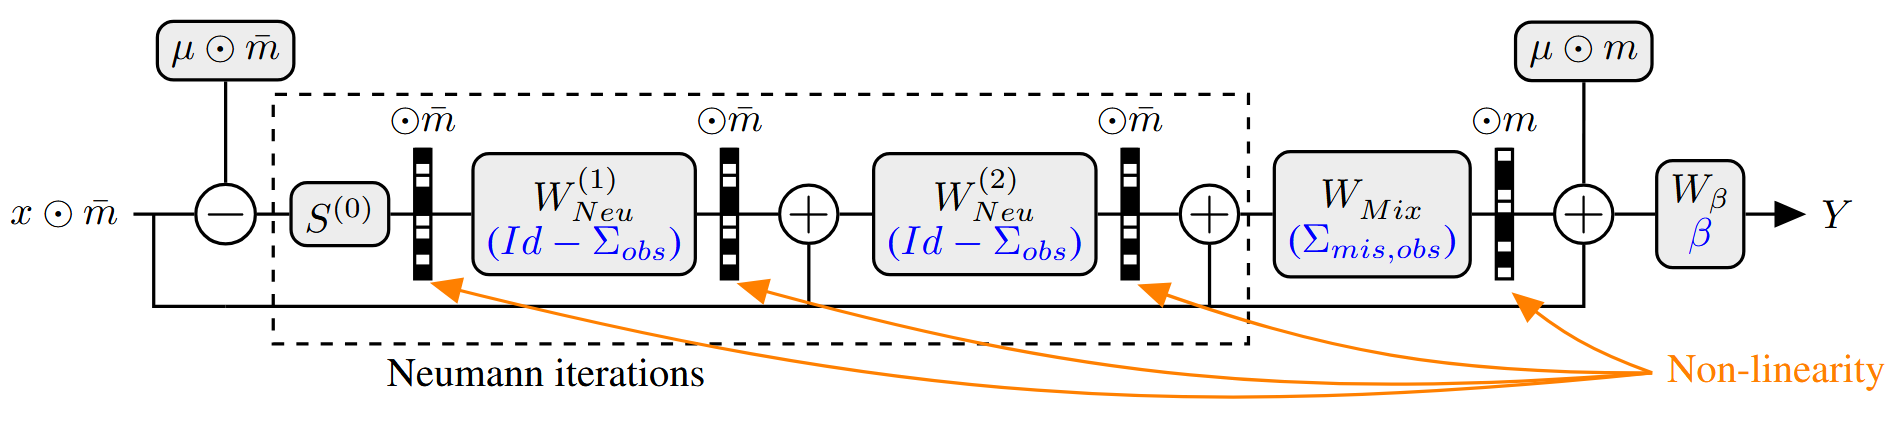
\includegraphics[width=\textwidth]{img/neumiss_network.png}
    \caption{
        \textbf{Kiến trúc mạng NeuMisss với độ sâu $4$} --- $\bar{m} = 1 - m$. Mỗi ma trận trọng số $W^{(k)}$ tương ứng với một phép biến đổi của \textcolor{blue}{ma trận hiệp phương sai}.
    }
    \label{fig:neumiss}
\end{figure}


Mỗi phép lặp Neumann đi qua một ma trận trọng số, qua tất cả $W^{(k)}_{Neu}$. Hay đúng hơn là ta học mỗi lớp một cách độc lập, theo như bài báo về Algorithm Unrolling \cite{gregor2010unroll} đã đề cập, khi mà các trọng số của các lớp có thể cải thiện hiệu quả xấp xỉ của mô hình.

Các trị số cho các giá trị quan sát được thay đổi với mỗi mẫu dữ liệu, nên 
có thể dẫn tới khó khăn trong việc cài đặt. 
Ví dụ như dữ liệu bị khuyết với mẫu $m$, ma trận trọng số $S^{(0)}, W_{Neu}^{(1)}, W_{Neu}^{(2)}$ của hình \ref{fig:neumiss} nên được masked sao cho các hàng và cột tương ứng với các trị số $mis(m)$ có giá trị bằng $0$, và các hàng của $W_{Mix}$ tương ứng với $obs(m)$ cũng như các cột của $W_{Mix}$ tương ứng với $mis(m)$ có giá trị bằng $0$.

Triển khai neural network với ma trận trọng số được masked theo các cách khác nhau với mỗi mẫu dữ liệu có thể phức tạp, nên bài báo đề xuất cách làm sau: Cho $W$ là ma trận trọng số, $v$ là một vector, và $\bar{m} = 1 - m$. Lúc này, $(W\odot \bar{m} \bar{m}^{\top}) v = (W(v \odot \bar{m}))\odot \bar{m}$, nghĩa là sử dụng ma trận trọng số được masked tương đương với việc masking vector đầu vào và đầu ra. Mạng NeuMiss có thể được xem là một neural network truyền thống với các hàm kích hoạt phi tuyến là \textbf{tích của các mask với nhau}. Cách tiếp cận này khiến việc cài đặt trở nên đơn giản hơn và cải thiện tốc độ tính toán của neural network, cũng như dễ dàng diễn giải hơn khi các mask điều khiển các thông tin của dữ liệu bị khuyết khi mạng được huấn luyện.

Theo như lý thuyết, chuỗi Neumann cần phải được lặp nhiều lần mới cho ra kết quả xấp xỉ nghịch đảo tốt, nên mạng NeuMiss cần phải sâu vì mỗi lớp tượng trưng cho 1 phép lặp. Do đó, mạng cần phải có residual connection, giúp model học được tốt hơn khi số lượng lớp nhiều.
Mặc dù sau khi thực nghiệm, việc có hay không có residual connection không ảnh hưởng quá nhiều đến hiệu suất của mạng NeuMiss (xem \ref{section:residual_connection}).


\textbf{Xấp xỉ trong trường hợp Gaussian self-masking}

Mặc dù kiến trúc mạng NeuMiss được xây dựng dựa trên dự đoán Bayes trong trường hợp MCAR và MAR, nhưng nó cũng có thể được sử dụng cho cơ chế self-masking~\eqref{eq:gaussian_bayes_predictor}. Giả sử $D_{mis} \cov_{mis|obs}^{-1} \approx Id$, thì dự đoán Bayes cho self-masking trở thành:
\begin{align*}
    f^*(X_{obs}, M) 
    &\approx \beta_{0}^{*} + \langle\beta_{obs}^{*}, X_{obs}\rangle 
    + \langle\beta_{mis}^{*},(2Id)^{-1} (\tilde{\mu}_{mis} + Id(\mu_{mis} + \cov_{mis,obs}\left(\cov_{obs}\right)^{-1} (X_{obs}-\mu_{obs}))) \rangle \\
    &\approx \beta_{0}^{*} + \langle\beta_{obs}^{*}, X_{obs}\rangle 
    + \langle\beta_{mis}^{*}, \frac{1}{2}(\tilde{\mu}_{mis} + \mu_{mis} + \cov_{mis,obs}\left(\cov_{obs}\right)^{-1} (X_{obs}-\mu_{obs})) \rangle \\
    &\approx \beta_0^* + \langle \beta_{obs}^*, X_{obs}\rangle + \langle \beta_{mis}^*, \frac{1}{2} (\widetilde{\mu}_{mis} + \mu_{mis}) + \frac{1}{2}  \cov_{mis,obs} (\cov_{obs})^{-1} (X_{obs} - \mu_{obs}) \rangle.
\end{align*}

Phương trình này giống như phương trình dự đoán Bayes cho cơ chế M(C)AR \eqref{eq:mcar_bayes_predictor}, nhưng với $\mu_{mis}$ được thay bởi $\frac{1}{2} (\widetilde{\mu}_{mis} + \mu_{mis})$ và $\cov_{mis,obs}$ trở thành $\frac{1}{2}\cov_{mis,obs}$. Dưới phép xấp xỉ này, dự đoán Bayes cho cơ chế self-masking có thể được mô hình bởi kiến trúc được đề xuất. Điểm khác biệt duy nhất là giá trị được quan tâm là tham số $\mu$ và $W_{mix}$ của mạng.

Một phép xấp xỉ khác cũng phù hợp cho dự đoán Bayes: $D_{mis} \cov_{mis|obs}^{-1} \approx \hat{D}_{mis}$ khi $\hat{D}$ là một ma trận ma trận đường chéo. Trong trường hợp này, kiến trúc được đề xuất có thể mô hình dự đoán Bayes cho self-masking:
\begin{multline*}
    f^*(X_{obs}, M) 
    \approx \beta_0^* + \langle \beta_{obs}^*, X_{obs}\rangle + \langle \beta_{mis}^*, 
    (Id + \hat{D}_{mis})^{-1} (\widetilde{\mu}_{mis} + \hat{D}_{mis} \mu_{mis}) \\
    + (Id + \hat{D}_{mis})^{-1} \hat{D}_{mis} \cov_{mis,obs} (\cov_{obs})^{-1} (X_{obs} - \mu_{obs}) \rangle.
\end{multline*}

Ở đây, tham số $\mu$ của mạng nhắm tới $(Id + \hat{D}_{mis})^{-1} (\widetilde{\mu}_{mis} + \hat{D}_{mis} \mu_{mis})$ và $W_{mix}$ nhắm tới $(Id + \hat{D}_{mis})^{-1} \hat{D}_{mis} \cov_{mis,obs}$ thay vì chỉ là $\cov_{mis,obs}$ trong trường hợp M(C)AR. Do đó, kiến trúc được đề xuất có thể xấp xỉ tốt dự đoán Bayes trong trường hợp self-masking bằng cách điều chỉnh giá trị tham số $\mu$ và $W_{mix}$ học được nếu $D_{mis} \cov_{mis|obs}^{-1}$ gần giống với ma trận đường chéo.



%-------------------------------------------------
% \section{Liên kết với MLP và hàm kích hoạt ReLU}
% % Multilayer Perceptron với hàm kích hoạt là 
% % hàm ReLU có dạng:
% % \begin{equation}
% %     \relu(x) = \max(x, 0).
% % \end{equation}

% % nhân các mask lại với nhau

% % Connections to Other Architectures:  A shallow (depth-1) NeuMiss network exhibits a close relationship to a Multilayer Perceptron (MLP) with ReLU activation that operates on the concatenated vector of imputed data and the mask.  This connection suggests that the commonly used MLP with an imputed mask can be interpreted as a simplified instance of a NeuMiss network.

% Một quy tắc thường dùng khi xử lý dữ liệu khuyết đó là xem dữ liệu đầu vào là ghép (concatenate) của dữ liệu với mask dữ liệu khuyết. Do  
% % the pattern of missing data itself may carry useful information for predictive models.
% các mẫu dữ liệu khuyết có thể cung cấp các thông tin hữu ích cho mô hình dự đoán.
% Mệnh đề tiếp theo liên kết quy tắc này với mạng NeuMiss.

% \begin{prop}(Mạng NeuMiss-1 layer tương đương với MLP)\label{prop:neumiss-mlp}
%     \newline
%     Cho $[X \odot (1-M), M] \in [0,1]^d \times \{0,1\}^d$ là dữ liệu đầu vào $X$ được điền khuyết bởi giá trị $0$ ghép với mask $M$.

%     \begin{itemize}
%         \item Cho $\mathcal{H}_{\relu} = (W \in \R^{d \times 2d}, \relu)$ là một hidden layer (layer ẩn) liên kết $[X \odot (1-M), M]$ với $d$ hidden units, và áp dụng hàm kích hoạt phi tuyến $\relu$.
%         \item Cho $\mathcal{H}_{\odot M} = (W \in \R^{d \times d}, \mu, \odot M)$ là một hidden layer liên kết $(X - \mu) \odot (1 - M)$ với $d$ hidden units, và áp dụng hàm kích hoạt phi tuyến $\odot M$.
%     \end{itemize}
%     Ký hiệu $h^{\relu}_{k}$ và $h^{\odot M}_{k}$ tượng trưng cho kết quả đầu ra của hidden unit thứ $k^{th}$ của mỗi layer. Thì tồn tại một tuỳ chỉnh của ma trận trọng số của hidden layer $\mathcal{H}_{\relu}$ sao cho $\mathcal{H}_{\odot M}$ và $\mathcal{H}_{\relu}$ có cùng hidden units kích hoạt cho bất kì $(X_{obs}, M)$, và hidden units được kích hoạt có dạng $h_{k}^{\relu}(X_{obs}, M) = h_{k}^{\odot M} (X_{obs}, M) + c_k$, với $c_k \in \R$.
% \end{prop}

% Mệnh đề 
% % \ref{prop:neumiss-mlp} 
% trên
% chỉ ra rằng, một hidden layer $\mathcal{H}_{\relu}$ có thể được viết lại như là một layer $\mathcal{H}_{\odot M}$ cộng với $1$ hằng số. Khi $1$ layer khác được thêm vào sau $\mathcal{H}_{\odot M}$ hay $\mathcal{H}_{\relu}$, hằng số này có thể được coi như là bias của layer mới này. Do đó, các trọng số của $\mathcal{H}_{\relu}$ có thể được học để giống với $\mathcal{H}_{\odot M}$. Trong trường hợp này, nó có nghĩa là một MLP với hàm kích hoạt \relu, với một hidden layer cho $d$  hidden units, hoạt động trên vector ghép với mask, thì giống với lại mạng NeuMiss với độ sâu là $1$ (Hình \ref{fig:neumiss}), do đó cung cấp một nền tảng lý thuyết cho việc sử dụng các mạng MLP sau mạng NeuMiss.

% \begin{proof}
%     Phần chứng minh có ở trong phần phụ lục A.7 của bài báo.
% \end{proof}

\section{Kết quả thực nghiệm}
Sau khi đã đi qua nền tảng lý thuyết của mạng NeuMiss, ta đi cài đặt và 
kiểm chứng các kết quả có đúng với lý thuyết hay không, dựa trên code của tác giả bài báo \footnote{Code của bài báo có tại \href{https://github.com/marineLM/NeuMiss}{https://github.com/marineLM/NeuMiss}}.

Toàn bộ code dùng để thực nghiệm trong bài báo cáo này được chạy trên Google Colab\footnote{\href{https://colab.research.google.com/}{https://colab.research.google.com/}},
có tại:
\href{https://github.com/ngntrgduc/seminar}{https://github.com/ngntrgduc/seminar}.


\subsection{Xấp xỉ ma trận bằng chuỗi Neumann}
Trước tiên, ta kiểm chứng độ hiệu quả cho việc xấp xỉ nghịch đảo ma trận nửa xác định dương, với bán kính phổ bé hơn $1$ bằng chuỗi Neumann.

\begin{figure}[h]
    \centering
    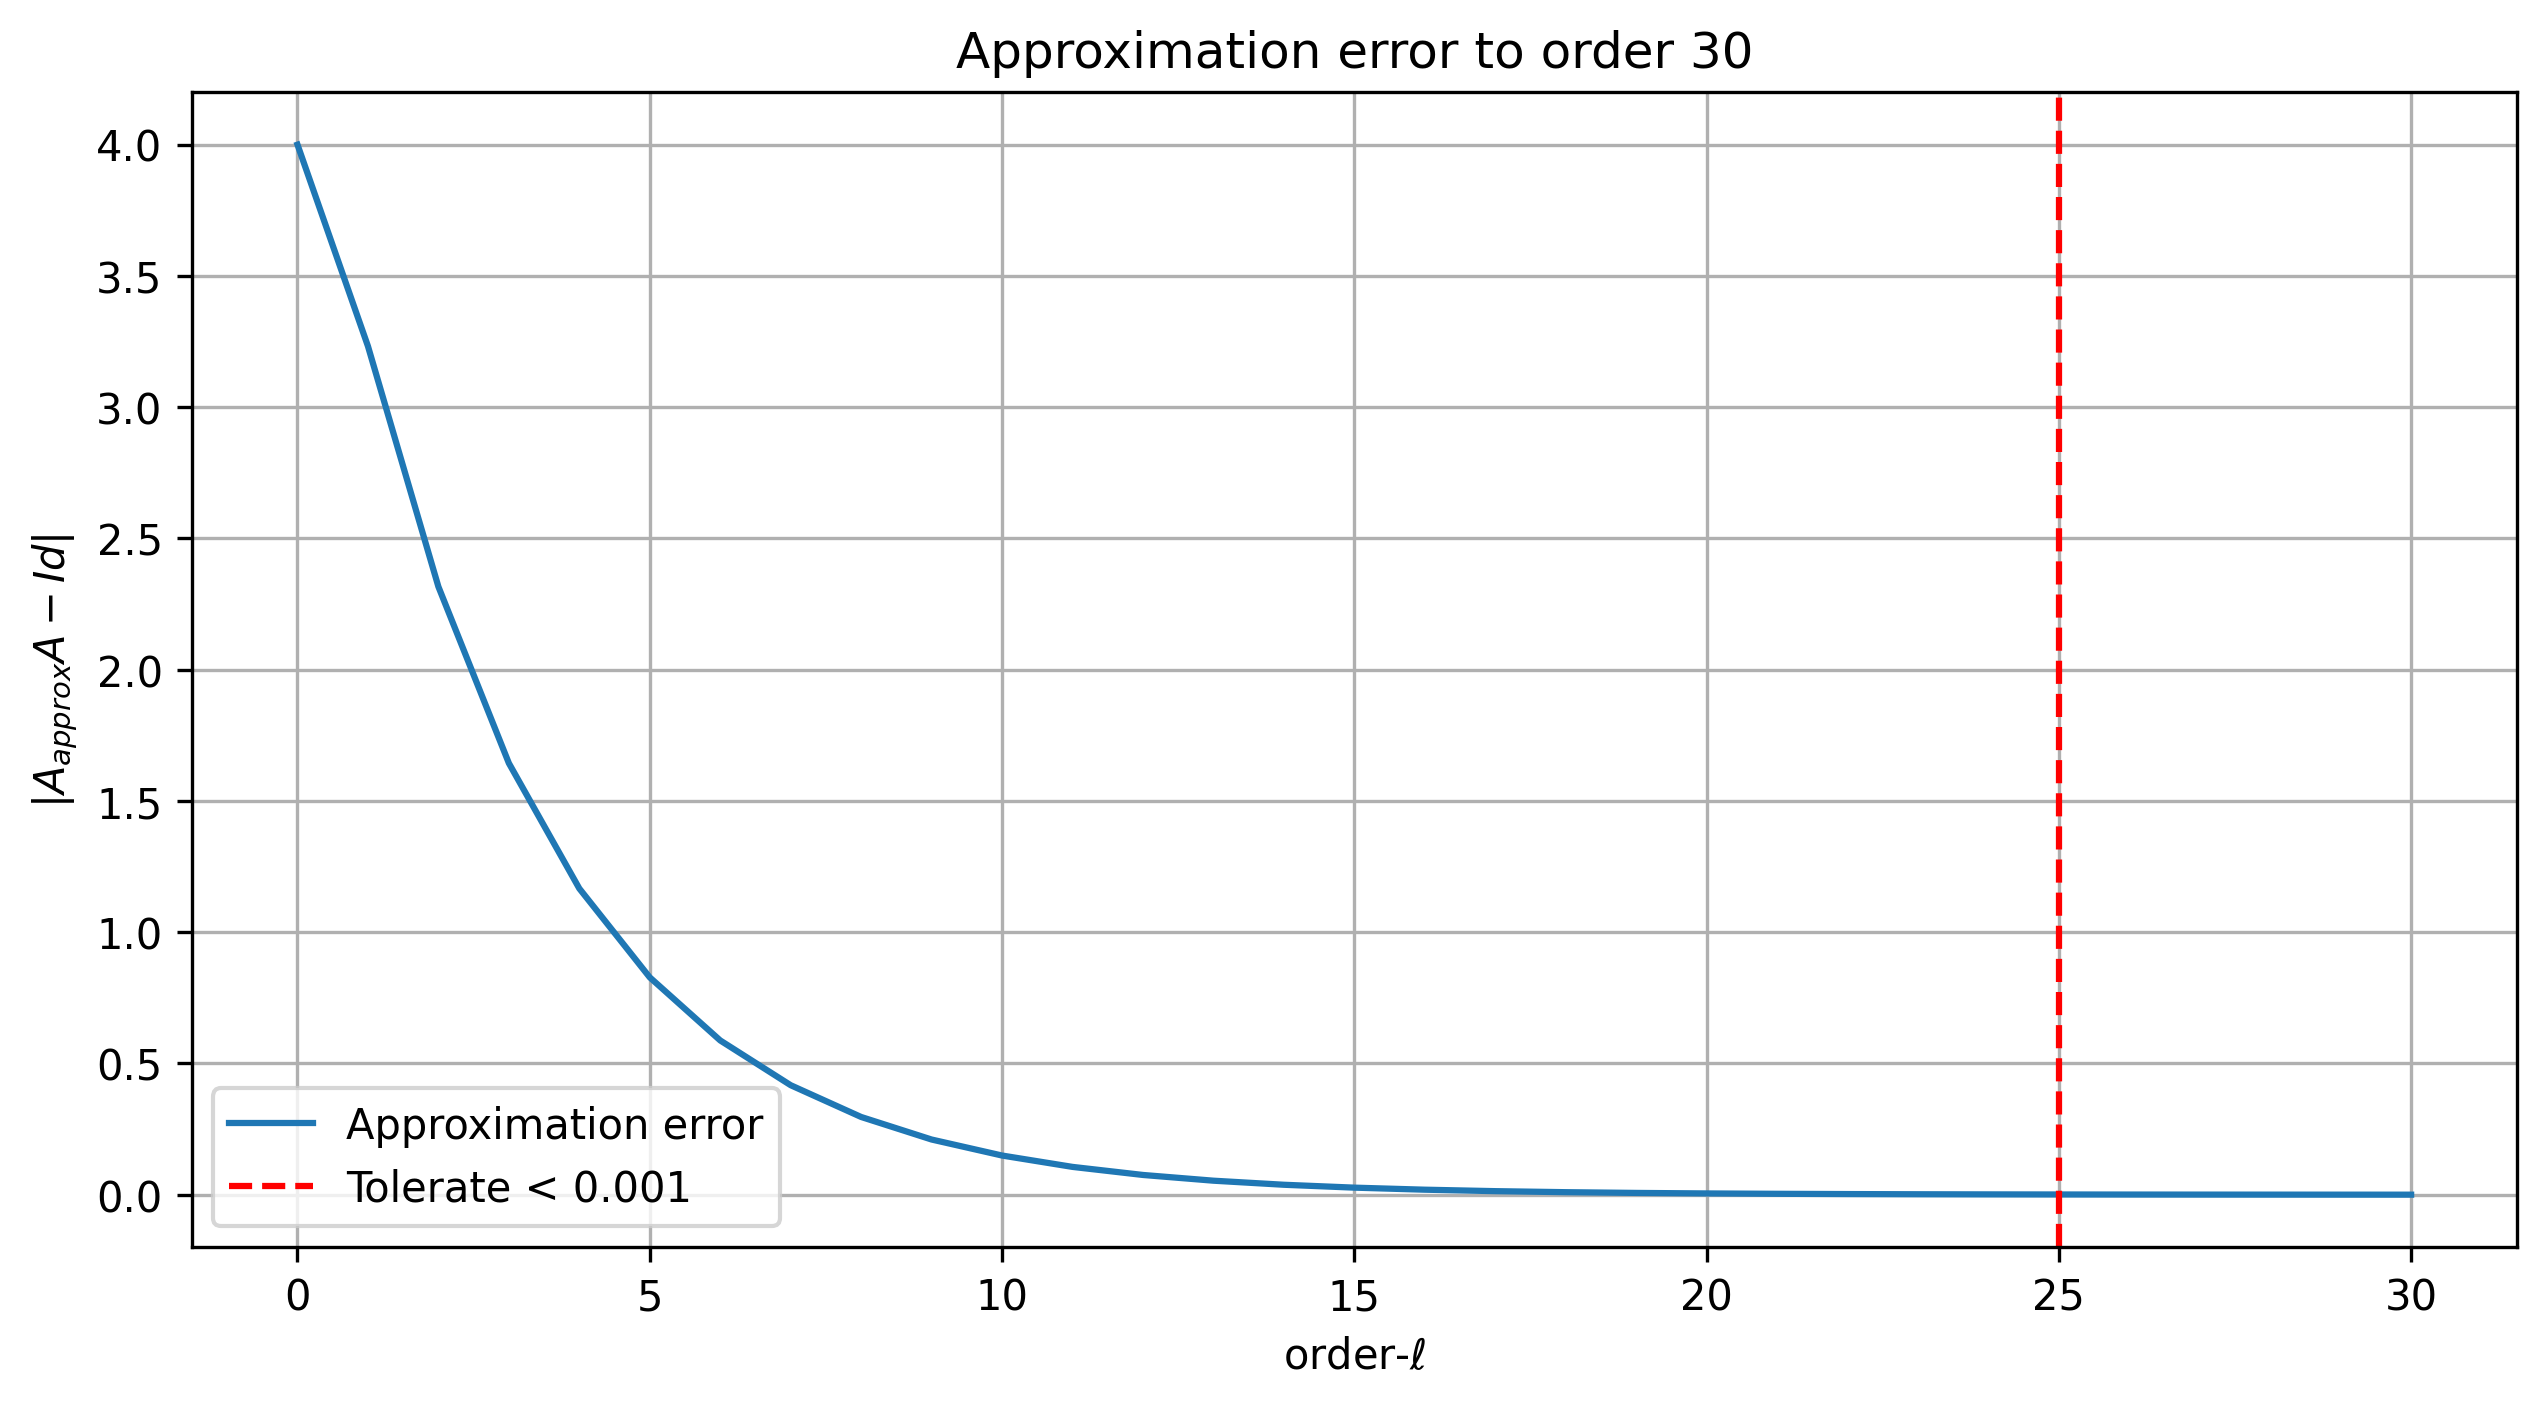
\includegraphics[width=.9\textwidth]{img/results/approx_neumann.png}
    \caption{
        Sai số của xấp xỉ ma trận tới bậc $30$.
    }
\end{figure}

Sử dụng $seed = 0$ như trong cài đặt của bài báo, ta có được một xấp xỉ nghịch đảo của ma trận tại bậc $25$ khá tốt khi mức sai số cho phép (tolerate) bé hơn $0.001$, mặc dù từ bậc $15$ thì sai số của xấp xỉ giảm không đáng kể. Sai số của xấp xỉ được tính bằng tổng sai khác của tích ma trận gốc và ma trận được xấp xỉ với lại ma trận đơn vị.
% np.sum(np.abs(np.dot(matrix, matrix_approx) - I))
    
Với các trường hợp bán kính phổ của ma trận lớn hơn $1$, chuỗi Neumann không hội tụ, nên không thể xấp xỉ ma trận được. Trong bài báo, dữ liệu được tạo ra với một ma trận hiệp phương sai với bán kính phổ lớn hơn $1$. Sở dĩ bài báo không quan tâm tới bán kính phổ lớn hơn $1$ 
là vì mạng NeuMiss sử dụng các ma trận trọng số để học và xấp xỉ sao cho các lớp ma trận trọng số sẽ tương ứng với xấp xỉ nghịch đảo $\cov_{obs}^{-1}$, không bắt buộc bán kính phổ ma trận hiệp phương sai nhỏ hơn $1$ để hoạt động. Nên trong code tạo dữ liệu của tác giả, không có điều kiện kiểm tra bán kính phổ nhỏ hơn $1$.


\subsection{Mạng NeuMiss}
Ta tiến hành kiểm tra độ hiệu quả của mạng NeuMiss trên tập dữ liệu 
được sinh ra từ phân phối chuẩn đa biến, với $Y$ được tính bằng hàm tuyến tính của $X$ như trong phương trình \eqref{eq:lr_matrix_notation}, cùng với $50\%$ dữ liệu bị khuyết ngẫu nhiên (MCAR) ở mỗi đặc trưng trong tập dữ liệu và nhiễu $\varepsilon$ tuân theo phân phối chuẩn với tỷ lệ signal-to-noise (SNR) bằng~$10$ (tỷ lệ nhiễu nhỏ hơn $10$ lần so với ``tín hiệu'' $Y$).

Do dữ liệu được sinh ra từ mô hình tuyến tính, nên bài báo sử dụng metric $R$ bình phương (R-squared -- $R^2$), hay còn được gọi là hệ số xác định (coefficient of determination), để tính 
tỷ lệ của độ biến thiên cho biến phụ thuộc $Y$ được giải thích bởi biến độc lập $X$, từ đó đánh giá độ hiệu quả của mô hình. 

Ngoài ra, ta còn có các biến thể khác của $R^2$ như:
\begin{itemize}
    \item $R^2$ hiệu chỉnh (Adjusted R-squared) cho ta biết được tỷ lệ biến thiên được giải thích chỉ bằng các biến độc lập thật sự ảnh hưởng tới biến phụ thuộc.
    \item $R^2$ cho dự đoán (Predicted R-Squared) cho biết độ chính xác của mô hình trên tập dữ liệu chưa biết.
\end{itemize}

Tuy nhiên, ta không quan tâm tới các mối quan hệ của các biến độc lập với biến phụ thuộc mà chỉ quan tâm tới độ tốt của mô hình trên tập dữ liệu đang xét, nên $R^2$ hiệu chỉnh hay $R^2$ cho dự đoán không được sử dụng trong trường hợp này.

Bayes rate (Tỷ lệ Bayes) là giá trị $R^2$ tốt nhất mà mô hình đạt được dựa trên lý thuyết, được ước lượng thông qua phương trình dự đoán Bayes \eqref{eq:lr_matrix_notation}.
Khi hệ số xác định càng gần với Bayes rate, tức kết quả $R^2 - \text{Bayes rate}$ càng tiến về $0$ thì độ hiệu quả của mô hình càng tốt. 


Sử dụng PyTorch để cài đặt mạng NeuMiss với độ sâu $10$, hàm mất mát là MSE, train (huấn luyện) trên CPU, thời gian train tầm $2$ phút cho 500~epochs, với batch size là~$256$, learning rate là 0.001.
Mạng cho ra chỉ số $R^2$ cho tập train quanh ngưỡng $0.8$, tập validation và test quanh ngưỡng $0.75$.

% Ngoài ra, tác giả chính của bài báo cũng cho ra thêm một bài báo nữa vào năm 2021 \cite{le2021goodimputation}, nói về việc có thể áp dụng NeuMiss cho các mô hình phi tuyến bằng cách huấn luyện nó chung với mô hình MLP sau mạng NeuMiss.


\begin{table}[h!]
\centering
\setlength{\tabcolsep}{10pt}
\begin{tabular}{lcccccc}
\toprule
& \multicolumn{2}{c}{\textbf{Train Set}} & \multicolumn{2}{c}{\textbf{Validation Set}} & \multicolumn{2}{c}{\textbf{Test Set}} \\
\cmidrule(lr){2-3}\cmidrule(lr){4-5}\cmidrule(lr){6-7}
 & $R^2$ & MSE & $R^2$ & MSE & $R^2$ & MSE \\
\midrule
NeuMiss depth-10 & 0.8072 & 0.208 & 0.7482 & 0.2808 & 0.7578 & 0.2674 \\
\bottomrule
\end{tabular}
\captionsetup{justification=centering, width=\linewidth}
\caption{Hiệu suất của NeuMiss với độ sâu 10.}
\label{tab:performance}
\end{table}
% Trong khi đó, Bayes rate cho tập train là $0.8205$ và tập test là $0.8078$. Ta thấy mạng NeuMiss cho ra kết quả khá tốt so với kết quả đạt được của mô hình 


\subsection{Một số kết quả khác}
Sau đây là một số kết quả thực nghiệm khác cho mạng NeuMiss, được train với 500 epochs.

\subsubsection*{So sánh mạng khi có residual connection với khi không có residual connection}\label{section:residual_connection}
Với mạng NeuMiss độ sâu 10:
\begin{table}[h!]
\centering
\setlength{\tabcolsep}{7.3pt}
\begin{tabular}{p{5.3cm}cccccc}
\toprule
& \multicolumn{2}{c}{\textbf{Train Set}} & \multicolumn{2}{c}{\textbf{Validation Set}} & \multicolumn{2}{c}{\textbf{Test Set}} \\
\cmidrule(lr){2-3}\cmidrule(lr){4-5}\cmidrule(lr){6-7}
 & $R^2$ & MSE & $R^2$ & MSE & $R^2$ & MSE \\
\midrule
\raggedright Có residual connection & 0.8116 & 0.2033 & 0.7424 & 0.2873 & 0.7511 & 0.2747 \\
\raggedright Không có residual connection & 0.8257 & 0.1880 & 0.7708 & 0.2556 & 0.7641 & 0.2604 \\
\bottomrule
\end{tabular}
\captionsetup{justification=centering, width=\linewidth}
\caption{Hiệu suất của NeuMiss với độ sâu 10 khi có và không có residual connection.}
\label{tab:performance_residual}
\end{table}

Khi không có residual connection, các chỉ số tốt hơn 1 chút so với khi có residual connection. Có thể do khi mạng có độ sâu lớn, việc có residual connection giúp mạng hoạt động hiệu quả hơn.

Qua đây, ta có thể thấy việc có residual connection không ảnh hướng nhiều tới kết quả so với mạng không có residual connection, như trong bài báo \cite{le2020neumiss} đã đề cập.


\subsubsection*{So sánh các mạng với độ sâu khác nhau}

\begin{table}[h!]
\centering
\setlength{\tabcolsep}{8pt}
\begin{tabular}{ccccccc}
\toprule
\textbf{Độ sâu} & \multicolumn{2}{c}{\textbf{Train Set}} & \multicolumn{2}{c}{\textbf{Validation Set}} & \multicolumn{2}{c}{\textbf{Test Set}} \\
\cmidrule(lr){2-3}\cmidrule(lr){4-5}\cmidrule(lr){6-7}
 & $R^2$ & MSE & $R^2$ & MSE & $R^2$ & MSE \\
\midrule
1  & 0.7823 & 0.2349 & 0.7500 & 0.2788 & 0.7678 & 0.2563 \\
5  & 0.7959 & 0.2202 & 0.7492 & 0.2796 & 0.7586 & 0.2664 \\
10 & 0.8191 & 0.1951 & 0.7548 & 0.2735 & 0.7676 & 0.2565 \\
15 & 0.8164 & 0.1980 & 0.7624 & 0.2650 & 0.7636 & 0.2610 \\
20 & 0.8157 & 0.1988 & 0.7286 & 0.3027 & 0.7431 & 0.2836 \\
\bottomrule
\end{tabular}
\captionsetup{justification=centering, width=\linewidth}
\caption{Hiệu suất của NeuMiss với các độ sâu khác nhau.}
\label{tab:performance-depths}
\end{table}

Mạng NeuMiss càng sâu thì hiện tượng hiệu suất giảm dần (diminishing returns) xuất hiện như trong bài báo \cite{le2020neumiss} đã đề cập. 
Điều này cho thấy việc tăng độ sâu của mạng không đảm bảo sẽ cải thiện kết quả trên tập test.


\subsubsection*{So sánh các mạng với tỷ lệ dữ liệu khuyết khác nhau}
\begin{table}[h!]
\centering
\setlength{\tabcolsep}{8pt}
\begin{tabular}{ccccccc}
\toprule
\textbf{Tỷ lệ khuyết} & \multicolumn{2}{c}{\textbf{Train Set}} & \multicolumn{2}{c}{\textbf{Validation Set}} & \multicolumn{2}{c}{\textbf{Test Set}} \\
\cmidrule(lr){2-3}\cmidrule(lr){4-5}\cmidrule(lr){6-7}
  & $R^2$ & MSE & $R^2$ & MSE & $R^2$ & MSE \\
\midrule
0.1\% & 0.8133 & 0.2014 & 0.7565 & 0.2716 & 0.7506 & 0.2752 \\
0.2\% & 0.8145 & 0.2001 & 0.7533 & 0.2751 & 0.7517 & 0.2741 \\
0.5\% & 0.8191 & 0.1952 & 0.7700 & 0.2565 & 0.7682 & 0.2558 \\
0.8\% & 0.7973 & 0.2187 & 0.7505 & 0.2782 & 0.7572 & 0.2680 \\
\bottomrule
\end{tabular}
\captionsetup{justification=centering, width=\linewidth}
\caption{Hiệu suất của NeuMiss độ sâu 10 với các tỷ lệ khuyết khác nhau.}
\label{tab:performance_missing_rates}
\end{table}

Ta nhận thấy rằng dù tỷ lệ khuyết nhiều nhưng NeuMiss vẫn cho ra kết quả tốt.


\subsubsection*{So sánh các mạng với số lượng mẫu và đặc trưng khác nhau}

\begin{table}[h!]
\centering
\setlength{\tabcolsep}{6pt}
\begin{tabular}{cccccccc}
\toprule
\textbf{Mẫu} & \textbf{Đặc trưng} & \multicolumn{2}{c}{\textbf{Train Set}} & \multicolumn{2}{c}{\textbf{Validation Set}} & \multicolumn{2}{c}{\textbf{Test Set}} \\
\cmidrule(lr){3-4}\cmidrule(lr){5-6}\cmidrule(lr){7-8}
 & & $R^2$ & MSE & $R^2$ & MSE & $R^2$ & MSE \\
\midrule
\multirow{2}{*}{100} & 10 & 0.8609 & 0.1581 & -1.6307 & 2.0416 & -12.7133 & 7.1884 \\
                     & 20 & 0.9450 & 0.0596 & -324.8323 & 205.5099 & -418.3801 & 224.8063 \\
\midrule
\multirow{2}{*}{1000} & 10 & 0.5976 & 0.4539 & -1.5842 & 2.8056 & -0.4908 & 1.6403 \\
                      & 20 & 0.7279 & 0.2953 & -42.1458 & 41.3359 & -64.2313 & 43.3147 \\
\midrule
\multirow{2}{*}{5000} & 10 & 0.8186 & 0.2037 & 0.7657 & 0.2481 & 0.7715 & 0.2491 \\
                      & 20 & 0.8929 & 0.1189 & -0.2029 & 1.3849 & -0.1616 & 1.3378 \\
\midrule
\multirow{2}{*}{10000} & 10 & 0.8138 & 0.2008 & 0.7489 & 0.2800 & 0.7568 & 0.2684 \\
                       & 20 & 0.8783 & 0.1336 & 0.1887 & 0.9035 & 0.2765 & 0.8806 \\
\midrule
\multirow{2}{*}{50000} & 10 & 0.8249 & 0.1933 & 0.8124 & 0.2071 & 0.8001 & 0.2232 \\
                       & 20 & 0.8056 & 0.2153 & 0.7145 & 0.3151 & 0.7282 & 0.3021 \\
\bottomrule
\end{tabular}
\captionsetup{justification=centering, width=\linewidth}
\caption{Hiệu suất của NeuMiss độ sâu 10 với các tuỳ chỉnh số lượng mẫu và đặc trưng khác nhau cho tập dữ liệu.}
\label{tab:performance_grouped_samples_features}
\end{table}

Qua Bảng \ref{tab:performance_grouped_samples_features}, ta thấy rằng mạng NeuMiss chỉ hoạt động tốt khi số lượng mẫu ở mức trung bình trở lên. Điều này cho thấy mạng NeuMiss phù hợp với các tập dữ liệu trung bình, như trong bài báo \cite{le2020neumiss} đã đề cập.


\subsubsection*{So sánh với các phương pháp khác}
Ta so sánh mạng NeuMiss với các phương pháp điền khuyết kết hợp việc sử dụng mô hình hồi quy tuyến tính để dự đoán. 
Các phương pháp này được cài đặt thông qua thư viện \textit{fancyimpute}\footnote{\href{https://pypi.org/project/fancyimpute/}{https://pypi.org/project/fancyimpute/}}, \textit{scikit-learn}\footnote{\href{https://pypi.org/project/scikit-learn/}{https://pypi.org/project/scikit-learn/}}, với kết quả tốt nhất được chọn từ nhiều tuỳ chỉnh khác nhau.
Các kết quả được so sánh với hiệu suất của mạng NeuMiss ở bảng \ref{tab:performance}, sử dụng chỉ số $R^2$ để đánh giá trên tập train và tập test. 

\begin{table}[h!]
\centering
\setlength{\tabcolsep}{10pt}
\begin{tabular}{lcc}
\toprule
& \multicolumn{1}{c}{\textbf{Train Set}} 
& \multicolumn{1}{c}{\textbf{Test Set}} \\
% \cmidrule(lr){2-3}\cmidrule(lr){4-5}\cmidrule(lr){6-7}
 % & $R^2$ & MSE & $R^2$ & MSE \\
\midrule
NeuMiss depth-10 & \textbf{0.8072}  & \textbf{0.7578} \\
KNN imputer + LR & 0.6929 & 0.7018 \\
Simple imputer + LR & 0.6574 & 0.6478 \\
SoftImpute + LR & 0.7604 & 0.7524 \\
MissForest + LR & 0.7708 & 0.7442 \\
MICE + LR & 0.7496 & 0.7313 \\
Simple imputer + MLP regressor & 0.8022 & 0.7330 \\

\bottomrule
\end{tabular}
\captionsetup{justification=centering, width=\linewidth}
\caption{Hiệu suất của NeuMiss độ sâu 10 với các phương pháp khác.}
\label{tab:performance-others}
\end{table}

Qua các kết quả này, ta có thể thấy mạng NeuMiss tỏ ra vượt trội hơn so với các phương pháp điền khuyết truyền thống.



% Tài liệu tham khảo
\newpage
\printbibliography[
    heading=bibintoc, % Add the bibliography to the ToC
    title={Tài liệu tham khảo}
]

% % \printindex

% Phụ lục
% \appendix

% \input{appendix/research-question}
% \input{appendix/roadmap}
% \input{appendix/proofs}

\end{document}

